%%================================================
%% Filename: chap03.tex
%% Encoding: UTF-8
%% Author: Yuan Xiaoshuai - yxshuai@gmail.com
%% Created: 2012-04-27 19:47
%% Last modified: 2016-08-28 21:08
%%================================================
\chapter{关于该模板的使用}
\label{cha:usage}

模板核心文件只有三个:\emph{zzuthesis.cls},\emph{zzuthesis.cfg} 和
\emph{zzubib.bst},其中定义的命
令分为两类:一是格式控制,二是内容替换。格式控制如字体、字号、字距和行距。内容
替换如姓名、院系、专业、致谢等等。模板自带的示例文档里面基本涵盖了论文写作用到
的所有命令及其使用方法,只需要用自己的内容进行相应替换就可以。本章将会对模板中
的命令及其使用作一简要介绍。

\section{\zzuthesis{} 示例文件}

下面的例子描述了模板中章节的组织形式,来自于示例文档,具体内容可以参考模板附
带的 \emph{main.tex} 和 \emph{data}\//。
\begin{code}
\documentclass[bachelor]{zzuthesis}
% \documentclass[%
%   bachelor|master|doctor, % mandatory option
%   openany|openright]{zzuthesis}

\usepackage{docutils}%模板文档用到的宏包及定义

\graphicspath{{figures/}}
\end{code}
\begin{code}
\begin{document}
\frontmatter
\tongjisetup{
  %******************************
  % 注意:
  %   1. 配置里面不要出现空行
  %   2. 不需要的配置信息可以删除
  %******************************
  %
  %=====
  % 秘级
  %=====
  secretlevel={保密},
  secretyear={2},
  %
  %=========
  % 中文信息
  %=========
  % 题目过长可以换行(推荐手动加入换行符,这样就可以控制换行的地方啦)。
  ctitle={同济大学学位论文 \LaTeX{} 模板\\使用示例说明与参考},
  cheadingtitle={同济大学学位论文 \LaTeX{} 模板使用示例说明与参考},    %用于页眉的标题,不要换行
  cauthor={同济人},  
  studentnumber={201804},
  cmajorfirst={工学},
  cmajorsecond={电子控制计算机},
  cdepartment={同济大学Linux用户组},
  csupervisor={陈杰 教授}, 
  % 如果没有副指导老师或者校外指导老师,把{}中内容留空即可,或者直接注释掉。
  cassosupervisor={裴刚 教授~(校外)}, % 副指导老师
  % 日期自动使用当前时间,若需手动指定,按如下方式修改:
  % cdate={\zhdigits{2018}年\zhnumber{11}月},
  % 没有基金的话就注释掉吧。
  cfunds={(本论文由我要努力想办法撑到两行的著名国家杰出青年基金 (No.123456789) 支持)},
  %
  %=========
  % 英文信息
  %=========
  etitle={A Simple Sample of Tongji Thesis\\ Using \tongjithesis{}}, 
  eauthor={Tongji Ren},
  emajorfirst={Gong Xue},
  emajorsecond={DianziControlComputerScience},
  edepartment={TONGJILUG},
  % 日期自动使用当前时间,若需手动指定,按如下方式修改:
  % edate={November,\ 2018},
  efunds={(Supported by the Natural Science Foundation of China for\\ Distinguished Young Scholars, Grant No.123456789)},    
  esupervisor={Prof. Jie Chen},
  eassosupervisor={Prof. Gang Pei (XiaoWai)}
  }

% 定义中英文摘要和关键字
\begin{cabstract}  
  论文的摘要是对论文研究内容和成果的高度概括。摘要应对论文所研究的问题及其研究目
  的进行描述,对研究方法和过程进行简单介绍,对研究成果和所得结论进行概括。摘要应
  具有独立性和自明性,其内容应包含与论文全文同等量的主要信息。使读者即使不阅读全
  文,通过摘要就能了解论文的总体内容和主要成果。

  论文摘要的书写应力求精确、简明。切忌写成对论文书写内容进行提要的形式,尤其要避
  免“第 1 章……;第 2 章……;……”这种或类似的陈述方式。

  本文介绍同济大学论文模板 \tongjithesis{} 的使用方法。本模板符合学校的硕士、
  博士论文格式要求。

  本文的创新点主要有:
  \begin{itemize}
    \item 用例子来解释模板的使用方法;
    \item 用废话来填充无关紧要的部分;
    \item 一边学习摸索一边编写新代码。
  \end{itemize}

  关键词是为了文献标引工作、用以表示全文主要内容信息的单词或术语。关键词不超过 5
  个,每个关键词中间用分号分隔。(模板作者注:关键词分隔符不用考虑,模板会自动处
  理。英文关键词同理。)
\end{cabstract}

\ckeywords{\TeX, \LaTeX, CJK, 模板, 论文}

\begin{eabstract}
   An abstract of a dissertation is a summary and extraction of research work
   and contributions. Included in an abstract should be description of research
   topic and research objective, brief introduction to methodology and research
   process, and summarization of conclusion and contributions of the
   research. An abstract should be characterized by independence and clarity and
   carry identical information with the dissertation. It should be such that the
   general idea and major contributions of the dissertation are conveyed without
   reading the dissertation.

   An abstract should be concise and to the point. It is a misunderstanding to
   make an abstract an outline of the dissertation and words ``the first
   chapter'', ``the second chapter'' and the like should be avoided in the
   abstract.

   Key words are terms used in a dissertation for indexing, reflecting core
   information of the dissertation. An abstract may contain a maximum of 5 key
   words, with semi-colons used in between to separate one another.
\end{eabstract}

\ekeywords{\TeX, \LaTeX, CJK, template, thesis}%封面
\makecover

% Abstract
\clearpage
\thispagestyle{plain}
\phantomsection
\addcontentsline{toc}{chapter}{Abstract}

\centerline{\zihao{3}\bfseries Abstract}

\linespread{1.4}\zihao{-4}
\bigskip

This thesis explores the relationship between focus structure and pronoun resolution among non-native speakers of English and French. Firstly we reviewed the existing literature on the mechanism of focus effect and pronoun resolution. Then through a self-paced reading test, we find that focus, in the form of cleft structure does not necessarily increase the salience of a informational unit, thus may not in some cases make it a preferred antecedent for pronoun resolution. This result is line with previous researches on this topic. In our experiment, We also find that focused subject in French and focused object in English are processed faster, but focused subjects in both languages leads to longer response time of anaphora. Furthermore, our research also shows that the congruence between anaphora and focus does not make the latter more accessible. In this regard, we argue that the problem of whether there is subject or object preference in English and French is more complicated than the results of current studies.

\bigskip
\noindent\textbf{\zihao{4} Keywords:} 
focus effect, pronoun resolution, self-paced reading, English, French

%摘要

\tableofcontents%目录
\listoffigures%插图清单
\listoftables%表格清单
\begin{denotation}
\begin{table}[h]%此处最好是h
\caption{国际单位制中具有专门名称的导出单位}
\vspace{0.5em}\centering\wuhao
\begin{tabular}{ccccc}
\toprule[1.5pt]
量的名称&单位名称&单位符号&其它表示实例\\
\midrule[1pt]
频率&赫[兹]&Hz&s-1\\
\bottomrule[1.5pt]
\end{tabular}
\end{table}
\end{denotation}
%符号列表
\end{code}
\begin{code}
\mainmatter
\chapter{绪论}
本章介绍了无线传感网的结构及其应用领域。分析规模化无线传感网的特点,对规模化传感网数据认证的需求和面临的挑战进行了分析。概述了本文的研究内容,并对文章的组织结构予以说明。
\section{本文研究背景和意义}
无线传感器网络(Wireless Sensor Networks,无线传感网)是一种特殊组织结构的移动自组网\upcite{c:sensor},在环境监测、工业控制、资源监控、智能家居、医疗保健和军事等各种领域都有广泛应用,有非常重要的地位和作用。
随着无线传感网技术的不断发展,很多应用进入了日常生活中,物联网技术也将成为未来发展的重要方向。
无线传感网的各种技术发展紧跟具体的应用需求,随着各种应用场景需要的安全性越来越高,安全问题也成为了阻碍无线传感网大规模发展的一个制约。

大范围监测在环境监测和军事侦察等诸多关系国家社会重大安全的领域都具有重要的地位和作用。在环境监测领域,往往面临范围野外受限甚至恶劣条件,在海洋等资源监测领域,水声通信等基础技术还不是很完善, 在军事侦察对抗领域更是要应对破坏攻击情况,传统的大范围实时监测机制和系统都难以得到有效部署,使用无线传感技术成为了最好的解决方案。规模化无线传感网因此应运而生,而且为满足大范围监测的需要,无线传感网的规模越来越大。

规模化无线传感网面临的安全威胁更多,攻击的影响更大,而且由于传感器节点的特点,传统的安全机制和协议无法直接适用于无线传感网,使得安全问题更加凸显。因此针对规模化无线传感网安全机制的研究成为了热门研究方向。

\subsection{无线传感网概述}
\subsubsection{无线传感网结构}
无线传感器节点被部署在目标监测区域,大量的传感器节点通过无线广播的方式,以一定的算法自组织成为一个多跳的无线网络。如图~\ref{fig:cluster}所示,是一个典型无线传感网的结构\upcite{c:cluster},由三部分组成:监测区域的传感器节点、与外部网络连接的网关或基站、远程数据中心。在监测区域的传感器节点一般通过算法组成若干的簇,每个簇通过簇头节点与其他簇或者基站通信,这样的方案节约了节点的能量。簇内节点收集到监测数据以后通过簇头节点的整合,形成报文通过一定的路径发送给基站,基站进一步通过外部网络设备,如互联网、卫星等将监测数据传输到远程数据中心。

\begin{figure}[htbp]
  \centering
  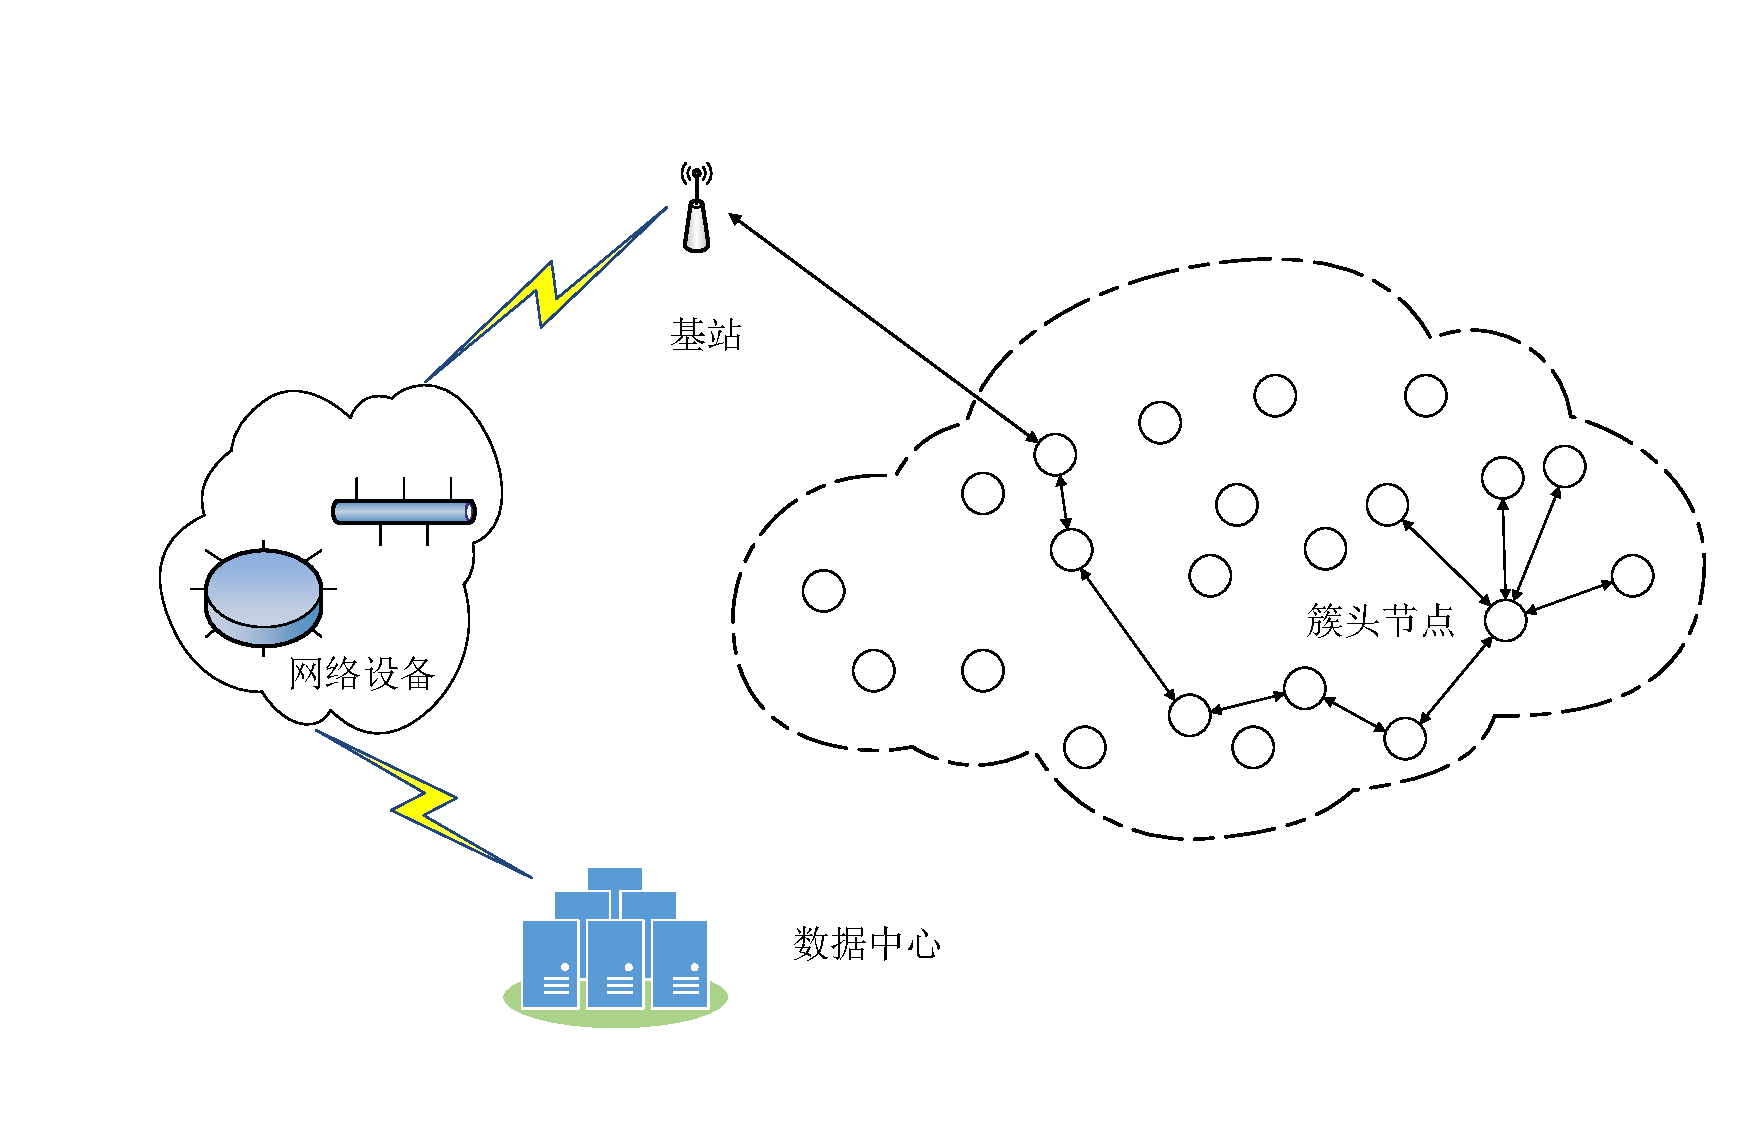
\includegraphics[width=5in]{cluster}
  \caption{无线传感网系统结构}
  \label{fig:cluster}
\end{figure}


无线传感网中,基站的计算和存储能力都比较强,
基站的功能可以是一个数据处理中心,向网络广播控制信息,从监测区域获取数据。
也可以是一个网络网关,负责数据向远程数据中心的传输。

\subsubsection{无线传感器节点结构}
传感器节点是无线传感网的基本组成单元,负责数据采集、发送等基本功能。
无线传感器节点一般仅具有很小的存储空间,较弱的计算能力,因此单个节点无法完成复杂的感知任务,需要大量的节点协同工作。

随着电子技术的发展,无线传感器节点的性能也有了很大的提升,如Crossbow公司研发的TelosB,CPU频率为8MHz,有10KB的RAM,使用2.4GHz无线电,能达到250Kbps数据传输,使用两节AAA电池(5号电池)供电。国产传感器节点典型的有美新的MEMSIC无线模块,工作频率可选433 MHz、868-915MHz或2.4GHz,拥有5年电池寿命,支持10-100米的发射范围,拥有19.2kbps-240kbps的数据传输速率。

\begin{figure}[htbp]
  \centering
  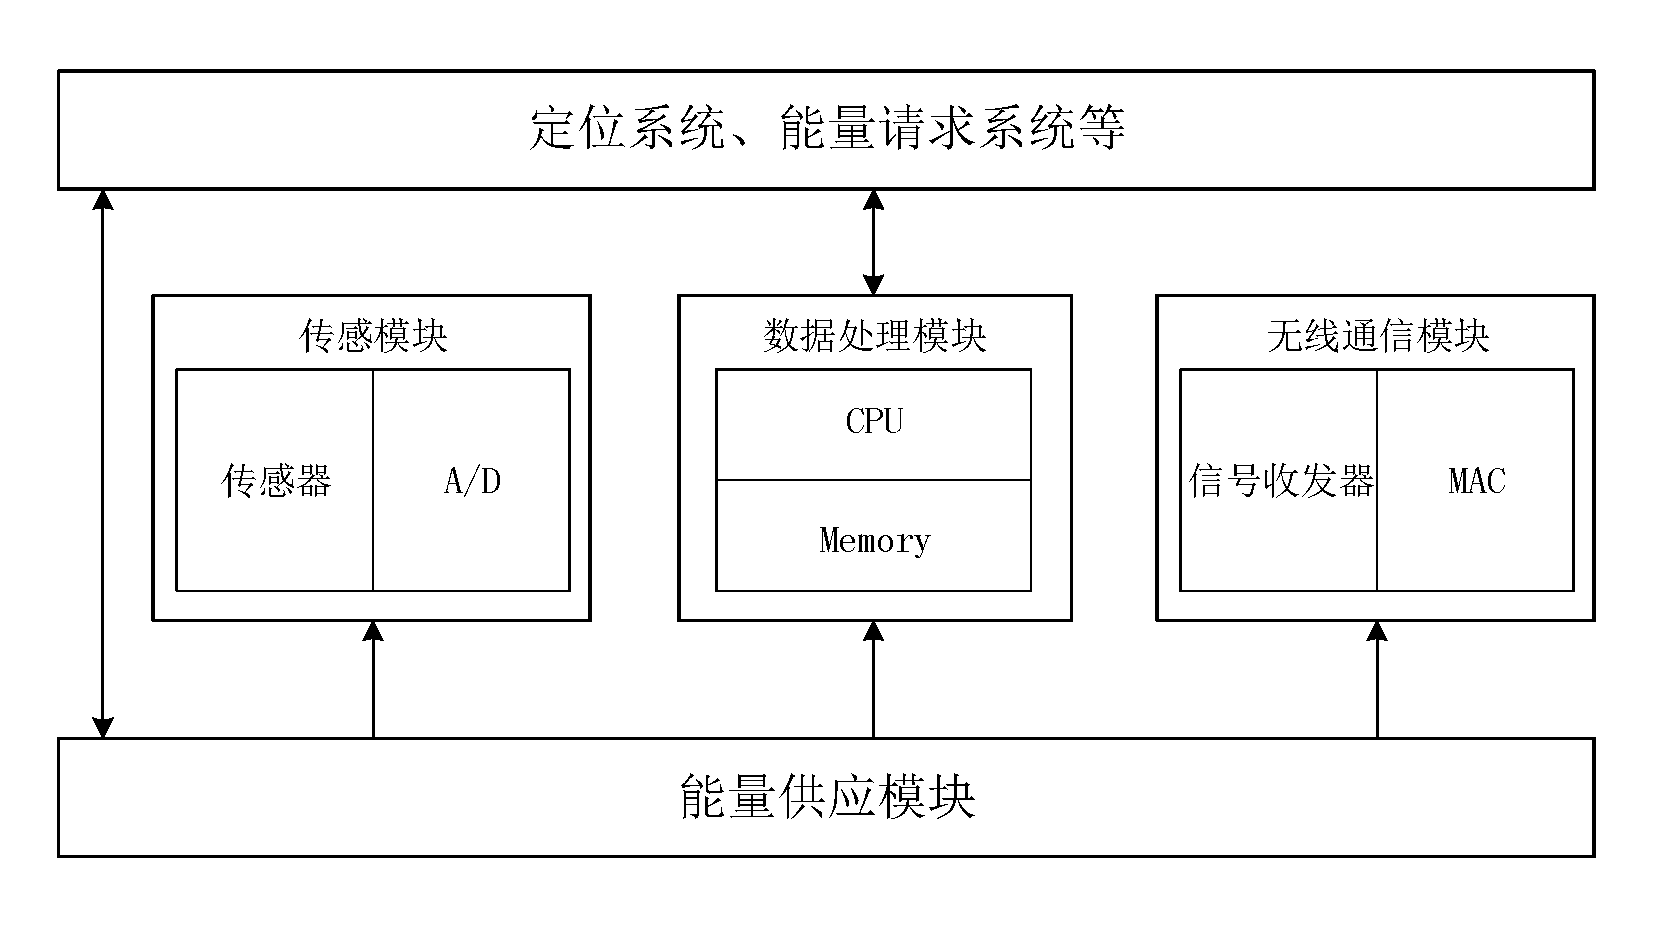
\includegraphics[width=5in]{node}
  \caption{无线传感网节点结构}
  \label{fig:node}
\end{figure}

这些传感器节点的设计原理基本相同,主要包括4个模块:传感模块、数据处理模块、无线通信模块和能量供应模块。
如图~\ref{fig:node}所示,是一个典型的无线传感器节点的结构图。传感模块主要负责从感知区域通过传感器获取数据,并将数据转化为适合进行网络传输的数字信号;数据处理模块主要包括处理和存储功能,负责控制传感器节点的运行,对传感模块获取的数据进行处理和存储,数据报文的整合与认证都是由数据处理模块完成,一般该模块需要嵌入式系统的支持,如UC Berkeley的开源嵌入式系统TinyOS\upcite{c:tinyos}等;无线通信模块负责与其他传感器节点或基站之间的通信,传感器节点一般使用内置天线进行数据收发;能量供应模块负责给其他模块供应能量,大部分传感器节点使用微型电池作为电源,因此能量非常有限。传感器节点中还包括一些负责定位、同步等功能的部件。

\subsubsection{无线传感网协议结构}

\begin{figure}[htbp]
  \centering
  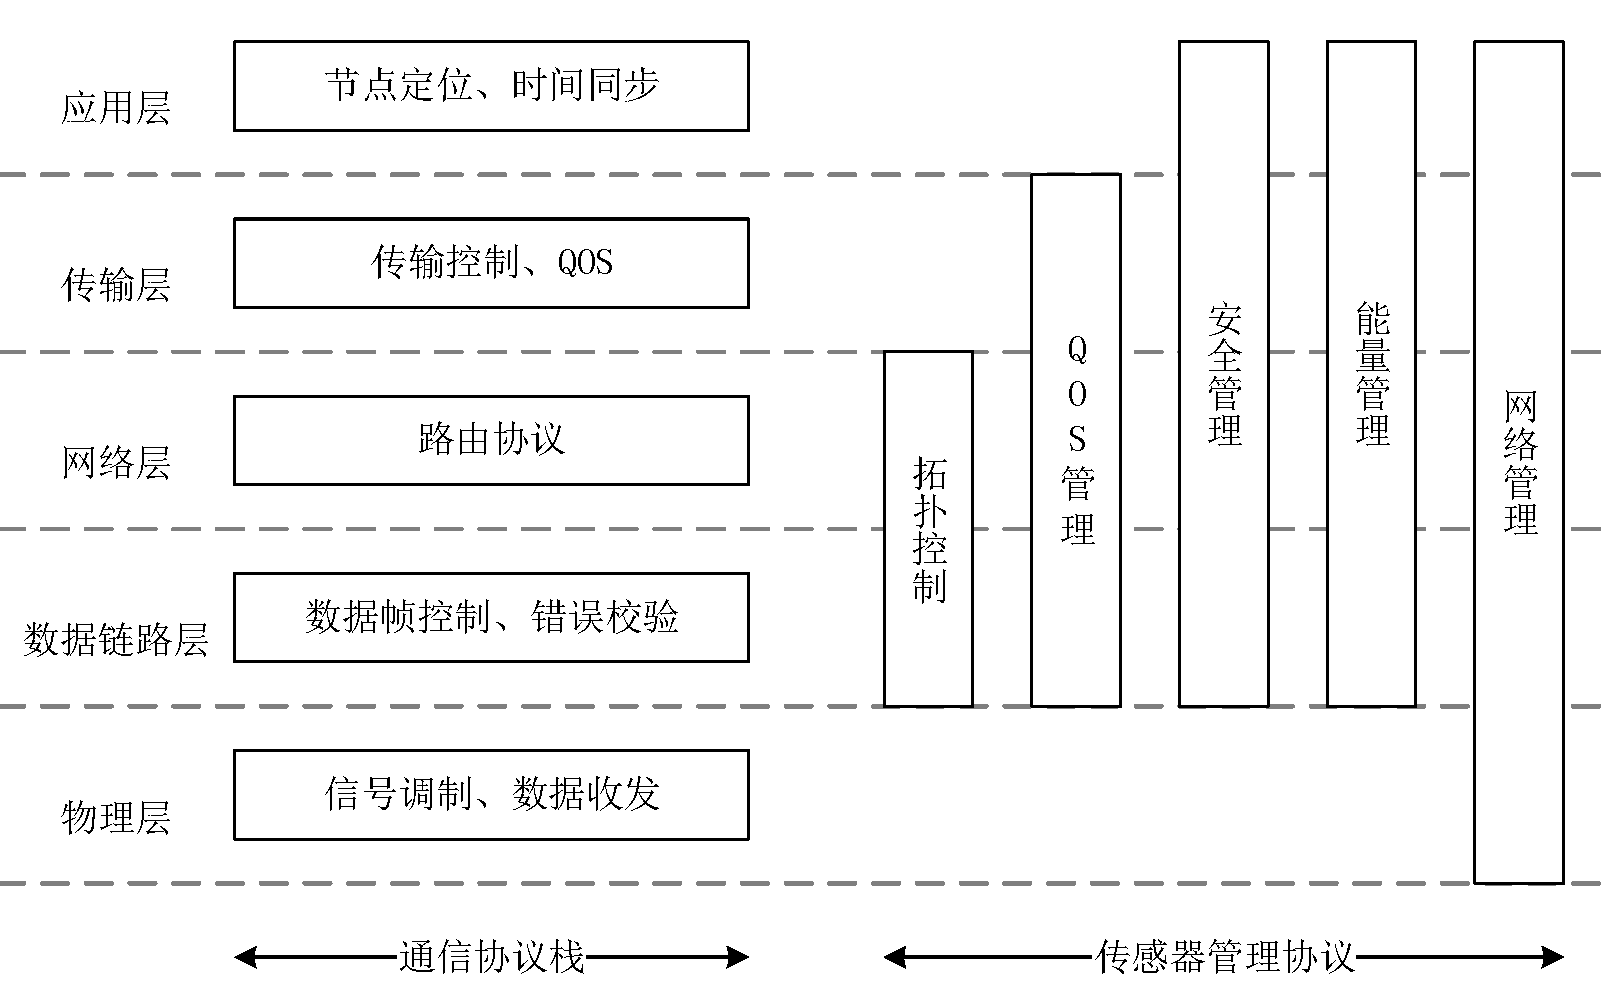
\includegraphics[width=5in]{construction}
  \caption{无线传感网协议结构}
  \label{fig:construction}
\end{figure}
无线传感网的通信协议栈和相关网络管理技术是当前的主要研究内容,协议结构如图~\ref{fig:construction}所示。
因为无线传感网是面向特定需求的网络,因此针对不同的部署环境,不同的网络部署结构,要对通信协议栈进行优化,使能量消耗、抗节点损耗、抗攻击能力等适应传感网的应用需求。

类似于OSI网络模型,无线传感网的通信协议栈由物理层、数据链路层、网络层、传输层、应用层组成:

物理层:物理层是通信协议栈的最底层,主要功能是将数据调制成适合传输的数字信号,通过无线电、红外灯无线介质完成传感器节点的数据收发。

数据链路层:数据链路层负责装配数据帧,对数据帧进行MAC校验,进行差错控制,向网络层提供透明可靠的数据传输服务。

网络层:主要负责无线传感网中的路由功能,将数据通过有效路径传送到目标节点,向传输层提供端对端的数据传输服务。

传输层:传输层负责数据报文的传送和控制,为应用层提供可靠的传输服务,对网络进行流量控制,进行服务质量控制(QOS)。

应用层:直接为应用提供服务,提供相应的应用协议和服务接口。

传感网管理协议提供了拓扑管理、QOS管理、安全管理、能量管理和网络管理等功能,实现对无线传感网以及各个节点的监控和管理。
\subsubsection{无线传感网的应用前景}
分布式传感网在军事中的应用是无线传感网的雏形,随着电子技术的不断发展,传感器节点的性能不断提升,无线传感网各种协议的完善和发展,使无线传感网在环境监测、军事侦察、智能家居、智能公路等各个领域得到了大量的应用,其应用前景十分广泛。

\begin{compactitem}
  \item 环境监测:无线传感网能完成大范围监测的任务,在自然数据采集中发挥重要作用,尤其是海洋监测传感网和内陆水文传感网等应用领域。如Li 等人将无线传感网部署在水产养殖水域,对水环境数据进行检测\upcite{c:water}。
  \item 军事侦察:由于无线传感网具有自组网、部署简单、容许节点失效等特点,适合部署在危险的敌对区域,完成军事侦察、战场环境监测等任务,因而在军事领域有很大应用前景,是现代化电子战的重要战略武器。如美国海军将开发的自主分布式DADS(Deployable Autonomous Distributed System)用于沿海广大海域的警戒、反潜和反水雷\upcite{c:DADS}。
  \item 智能家居:智能家居是通过无线传感器将房间中的各种家电等设备连接起来,实现家居环境的监测以及远程控制,构建出智能的居住环境\upcite{c:homes}。
  \item 智能公路:通过部署在公路上的无线传感器节点以及车载传感器节点,共同组成智能公路传感网络,对交通状况实现自动监测,引导车流等,实现自动化的公路交通管理。
\end{compactitem}



\subsection{规模化无线传感网数据认证}
\subsubsection{规模化无线传感网的特点}
规模化无线传感网是为满足大范围监测的需要而产生的,如国内著名的绿野千传项目,在浙江省天目山建立的大规林业监测传感网,部署的自组织传感网节点超过2000个,网络中传输路径跳数超过 20 跳
\upcite{c:lvye}。
规模化无线传感网具有如下的特点:
\begin{enumerate}\setlength{\itemsep}{-\itemsep}
  \item 节点数量大,覆盖面积广,节点失效较为频繁,网络拓扑结构相对不稳定。
  \item 一般部署于恶劣区域,甚至是敌对攻击区域,恶意攻击的频度增加。
  \item 节点的计算和存储能力更为受限,网络的能量较为敏感,对机制的轻量化要求更突出。
\end{enumerate}

\subsubsection{规模化无线传感网的数据认证需求}
无线传感网中的认证包括身份认证和数据认证。身份认证是对网络中节点的合法身份的一种判定机制,是数据认证的基础。无线传感网数据认证主要包括两个方面:
\begin{compactitem}
  \item 数据来源合法性,主要以身份认证为基础,通过数据报文中的认证机制判定数据报文的来源的合法性。
  \item 数据完整性,通过数据认证的机制,确保节点收到的数据报文没有被非法进行篡改。
\end{compactitem}

在环境监测等领域,规模化传感网每天都会产生海量的感知数据。在军事侦察领域,随着侦察区域的扩大,侦察精度的提高,传感网感知的数据量飞速增长。尤其在实时监测场景,数据量大、传输实时性要求高,无线传感器节点的性能限制使得规模化传感网实现可靠传输具有非常的难度,合适的数据认证机制可以为其提供有力支持。在无线传感网中数据泄露、错误数据甚至虚假数据会对网络的安全造成重大影响。尤其在重要战略场景或军事场景,还要考虑破坏攻击的可能,因此数据认证更为安全攸关。
\subsubsection{规模化无线传感网数据认证面临的挑战}

复杂环境下数据高安全性要求对数据认证提出的挑战。实时监测传感网通常部署环境恶劣,而且缺乏基础设施的建设,由于自然环境和主动攻击等对节点的破坏,使节点的失效率很高,网络拓扑结构动态变化,数据传输质量不够稳定,而且存在突发大故障潜因,需要在容灾抗毁前提下进行数据认证,确保传输的安全性。

端对端传输为数据认证提出的挑战。完全依靠广播等数据传输机制,在规模化无线传感网中,传输效率过低,消耗的节点能量和通信资源过大,而且容易受到泛洪攻击的影响。有效利用规模化传感网中端对端数据传输,能够有效的保证传输效率。在端对端传输中,由于多跳传输的原因,当路径中出现妥协节点时,整条路径容易被攻破,从而造成数据传输被攻击,因而在多路径端对端的数据传输中,有效利用数据认证机制加强路径上的安全保障是安全传输的关键。

轻量级认证机制及其实现技术为数据认证提出的挑战。规模化无线传感网传输的数据量大,要求处理快捷。在节点资源能力受限,通信能耗受限的前提下,需要计算、存储、通信都轻量级的水平,保障网络安全、传输可靠性、高效性和数据可信,具有很大难度。传统的的认证机制使用的密码算法复杂度未达到轻量级,不适合规模化传感网网络资源受限的特点,我们需要设计适合实时性较高的规模无线传感网达到轻量级算法。

攻击对抗对数据认证提出的挑战。无线传感网一般部署在恶劣环境中,而且具有自组网络的多跳性、无中心性和自组织性等特征,致使其通信协议栈的各个层级都容易遭受到各种形式的攻击,我们需要设计能够适应有限节点能量,有限计算能力的数据认证算法,对抗各种攻击,保证无线传感网传输数据的来源合法性和完整性。

\section{本文研究内容}
本文根据规模化无线传感网的安全需求以及其特点,针对其数据认证关键技术展开研究,使用多节点联合的技术思路研究数据认证模型和机制,并设计实现了关键算法。
主要工作如下:

\begin{enumerate}\setlength{\itemsep}{-\itemsep}
  \item 提出了多跳长路径上多节点联合数据认证的模型,设计了多跳长路径上多节点联合数据认证协议,并设计了路径上节点关系的维护算法,对协议的安全性能进行了分析评价。
  \item 针对多跳长路径上多写点联合数据认证协议的不足,对算法进行了优化,提出了多路径抗节点失效机制和动态步长多节点联合数据认证机制,并对优化方案的安全性能进行了分析评价。
  \item 围绕多跳长路径多节点联合数据认证机制的需求,对密钥分配方案进行了深入研究,提出了基于单向hash链的密钥分配方案,并对认证中的MAC进行了研究,提出了适应数据认证机制需求的MAC码。
\end{enumerate}


\section{本文组织结构}
本文一共分为七章。

第一章\quad 绪论,介绍了课题的选题背景,描述了无线传感网的特点,介绍了无线传感网的相关安全技术,列出了本文的主要研究内容和本文组织结构。

第二章\quad 相关研究概述,本章首先对无线传感网的安全技术进行了概述,然后重点对数据认证和密钥分配两种安全技术进行了论述。

第三章\quad 多跳长路径上多节点联合数据认证,本章提出了无线传感网中多跳长路径多节点联合的数据认证模型,及其设计目标。
重点介绍了关键算法与协议的设计实现,对多节点联合数据认证机制的安全性能进行了分析评价。

第四章\quad 数据认证方案优化,本章针对多跳长路径上多节点联合数据认证进行了优化,提出了多路径抗节点失效和动态步长多节点联合数据认证两个优化方案,并对它们的安全性能进行了分析评价。

第五章\quad 密钥分配与MAC设计,本章对多节点联合数据认证中的密钥分配方案以及使用的MAC的设计进行了介绍,提出了基于单向hash链的密钥分配方案,以及适应多节点联合数据认证的MAC码。

第六章\quad 仿真实验与结果分析,本章在仿真平台上对多跳长路径多节点联合数据认证机制,以及其优化方案进行了仿真实验,对它们的安全性能结果进行了评价。

第七章\quad 总结与展望,本章对全文的工作做了总结,指出了数据认证机制现阶段的不足以及未来研究中需要研究及完善的地方。

%正文章节
\chapter{中华人民共和国}
\label{cha:china}

\section{图的例子}
\label{sec:other}

在第~\ref{cha:intro} 章中我们学习了贝叶斯公式~(\ref{equ:chap1:bayes}),这里我们复
习一下:
\begin{equation}
\label{equ:chap2:bayes}
p(y|\mathbf{x}) = \frac{p(\mathbf{x},y)}{p(\mathbf{x})}=
\frac{p(\mathbf{x}|y)p(y)}{p(\mathbf{x})}
\end{equation}

\subsection{绘图}
\label{sec:draw}

本模板不再预先装载任何绘图包(如 \textsf{pstricks,pgf} 等),完全由你自己来决定。
个人觉得 \textsf{pgf} 不错,不依赖于 Postscript。此外还有很多针对 \LaTeX{} 的
 GUI 作图工具,如 XFig(jFig), WinFig, Tpx, Ipe, Dia, Inkscape, LaTeXPiX,
jPicEdt, jaxdraw 等等。

\subsection{插图}
\label{sec:graphs}
关于子图形的使用细节请参看 \textsf{subcaption} 的说明文档。

\subsection{一个图形}
\label{sec:onefig}
一般图形都是处在浮动环境中。之所以称为浮动是指最终排版效果图形的位置不一定与源文
件中的位置对应\footnote{This is not a bug, but a feature of
\LaTeX!},这也是刚使 用 \LaTeX{}
同学可能遇到的问题。如果要强制固定浮动图形的位置,请使用
\textsf{float} 宏包, 它提供了 \texttt{[H]}
参数,比如图~\ref{fig:heythere}。
\begin{figure}[H] % use float package if you want it here
  \centering
  
\includegraphics[height=2cm]{hello.jpg}
  \caption{插个图插个图}
  \label{fig:heythere}
\end{figure}

大学之道,在明明德,在亲民,在止于至善。知止而后有定;定而后能静;静而后能安;安
而后能虑;虑而后能得。物有本末,事有终始。知所先后,则近道矣。古之欲明明德于天
下者,先治其国;欲治其国者,先齐其家;欲齐其家者,先修其身;欲修其身者,先正其心;
欲正其心者,先诚其意;欲诚其意者,先致其知;致知在格物。物格而后知至;知至而后
意诚;意诚而后心正;心正而后身 修;身修而后家齐;家齐而后国治;国治而后天下
平。自天子以至于庶人,壹是皆以修身为本。其本乱而未治者 否矣。其所厚者薄,而其所
薄者厚,未之有也!

\hfill \pozhehao《大学》


\subsection{简单子图}
\label{sec:multifig}

如果多个图形相互独立,并不共用一个图形计数器,那么用 \verb|minipage| 或者
\verb|parbox| 就可以。否则,请参看图~\ref{fig:big1},它包含两个小图,分别是图~\ref{fig:subfig1}
和图~\ref{fig:subfig2}。推荐使用 \verb|\subcaption|,不要再用\verb|\subfloat|,\verb|\subfigure| 和 \verb|\subtable|了。
\begin{figure} %[h]
  \centering%
  \subcaptionbox{第一个小图形\label{fig:subfig1}}{%    
    
\includegraphics[height=2cm]{tongji-fig-logo.png}}\hspace{4em}%
  \subcaptionbox{第二个小图形。如果标题很长的话,它会自动换行,这个 caption 就是这样的例子\label{fig:subfig2}}{%    
    
\includegraphics[height=2cm]{tongji-text-logo.png}}
  \caption{包含子图形的大图形}
  \label{fig:big1}
\end{figure}

古之学者必有师。师者,所以传道受业解惑也。人非生而知之者,孰能无惑?惑而不从师,
其为惑也,终不解矣。生乎吾前,其闻道也固先乎吾,吾从而师之;生乎吾後,其闻道也亦
先乎吾,吾从而师之。吾师道也,夫庸知其年之先後生於吾乎!是故无贵无贱无长无少,道
之所存,师之所存也。

嗟乎!师道之不传也久矣,欲人之无惑也难矣。古之圣人,其出人也远矣,犹且从师而问焉;
今之众人,其下圣人也亦远矣,而耻学於师。是故圣益圣,愚益愚。圣人之所以为圣,愚
人之所以为愚,其皆出於此乎?爱其子,择师而教之,於其身也,则耻师焉,惑焉。彼童子
之师,授之书而习其句读者,非吾所谓传其道、解其惑者也。句读之不知,惑之不解,或师
焉,或不焉,小学而大遗,吾未见其明也。巫医、乐师、百工之人不耻相师,  士大夫之族
曰“师”曰“弟子”之云者,则群聚而笑之。问之,则曰:彼与彼年相若也,道相似也,位
卑则足羞,官盛则近谀。呜呼!师道之不复,可知矣。巫医、乐师、百工之人。吾子不齿,
今其智乃反不能及,其可怪也欤!圣人无常师。孔子师郯子、苌子、师襄、老聃。郯子之徒,
其贤不及孔子。孔子曰:“三人行,必有我师。”是故弟子不必不如师,师不必贤於弟子。
闻道有先後,术业有专攻,如是而已。

\subsection{复杂子图要注意遮挡}
使用子图的方法如图~\ref{fig:chap2:zitu}所示,使用\texttt{subcaptionbox}环境设置每一个子图,注意\texttt{subcaptionbox}其后需要有括号,以及子图换行时需要使用\texttt{vskip},以免下一排子图会对上一排子图的图名造成遮挡。
\begin{figure}[htbp]
\centering
  \subcaptionbox{第一个小图形}{\label{fig:chap1:zitu:a}
  
\includegraphics[width=5cm]{tongji-fig-logo}\hskip2cm}
  \subcaptionbox{第二个小图形}{\label{fig:chap1:zitu:b}
  
\includegraphics[width=5cm]{tongji-fig-logo}}
\vskip0.5cm
  \subcaptionbox{第三个小图形}{\label{fig:chap1:zitu:c}
  
\includegraphics[width=5cm]{tongji-fig-logo}\hskip2cm}
  \subcaptionbox{第四个小图形}{\label{fig:chap1:zitu:d}
  
\includegraphics[width=5cm]{tongji-fig-logo}}
\caption{多子图用\texttt{subcaptionbox}}\label{fig:chap2:zitu}
\end{figure}


\subsection{多个图形独立}
如果要把编号的两个图形并排,那么小页就非常有用了,如图~\ref{fig:parallel2}:
\begin{figure}
\begin{minipage}{0.48\textwidth}
  \centering
  
\includegraphics[height=2cm]{tongji-whole-logo.png}
  \caption{并排第一个图}
  \label{fig:parallel1}
\end{minipage}\hfill
\begin{minipage}{0.48\textwidth}
  \centering
  
\includegraphics[height=2cm]{tongji-whole-logo.png}
  \caption{并排第二个图}
  \label{fig:parallel2}
\end{minipage}
\end{figure}


李氏子蟠,年十七,好古文、六艺,经传皆通习之,不拘於时,学於余。余嘉其能行古
道,作师说以贻之。

\hfill \pozhehao 韩愈(唐)


\subsection{插图大原则}
同志们,如果遇到问题一定要会搜索,要么看别人的问答,要么看宏包的文档,希望你不要成为重度伸手党。
一点微小的工作,谢谢大家。

\section{插入pdf格式图片的问题}
\label{sec:problem}
在\LaTeX{}中插入高清图片一般有两种方式:1)插入~eps~矢量图,2)插入~pdf~格式图片。在模板测试过程中遇到一个插入
~pdf~格式图片的问题。

问题描述

插入~pdf~格式的图,有时采用~XeLaTeX~编译后,插图被翻转~90~度。有时却不会出现该问题。问题图片如图~\ref{rotatedBode}~所示。
\begin{figure}[H] 
  \centering
  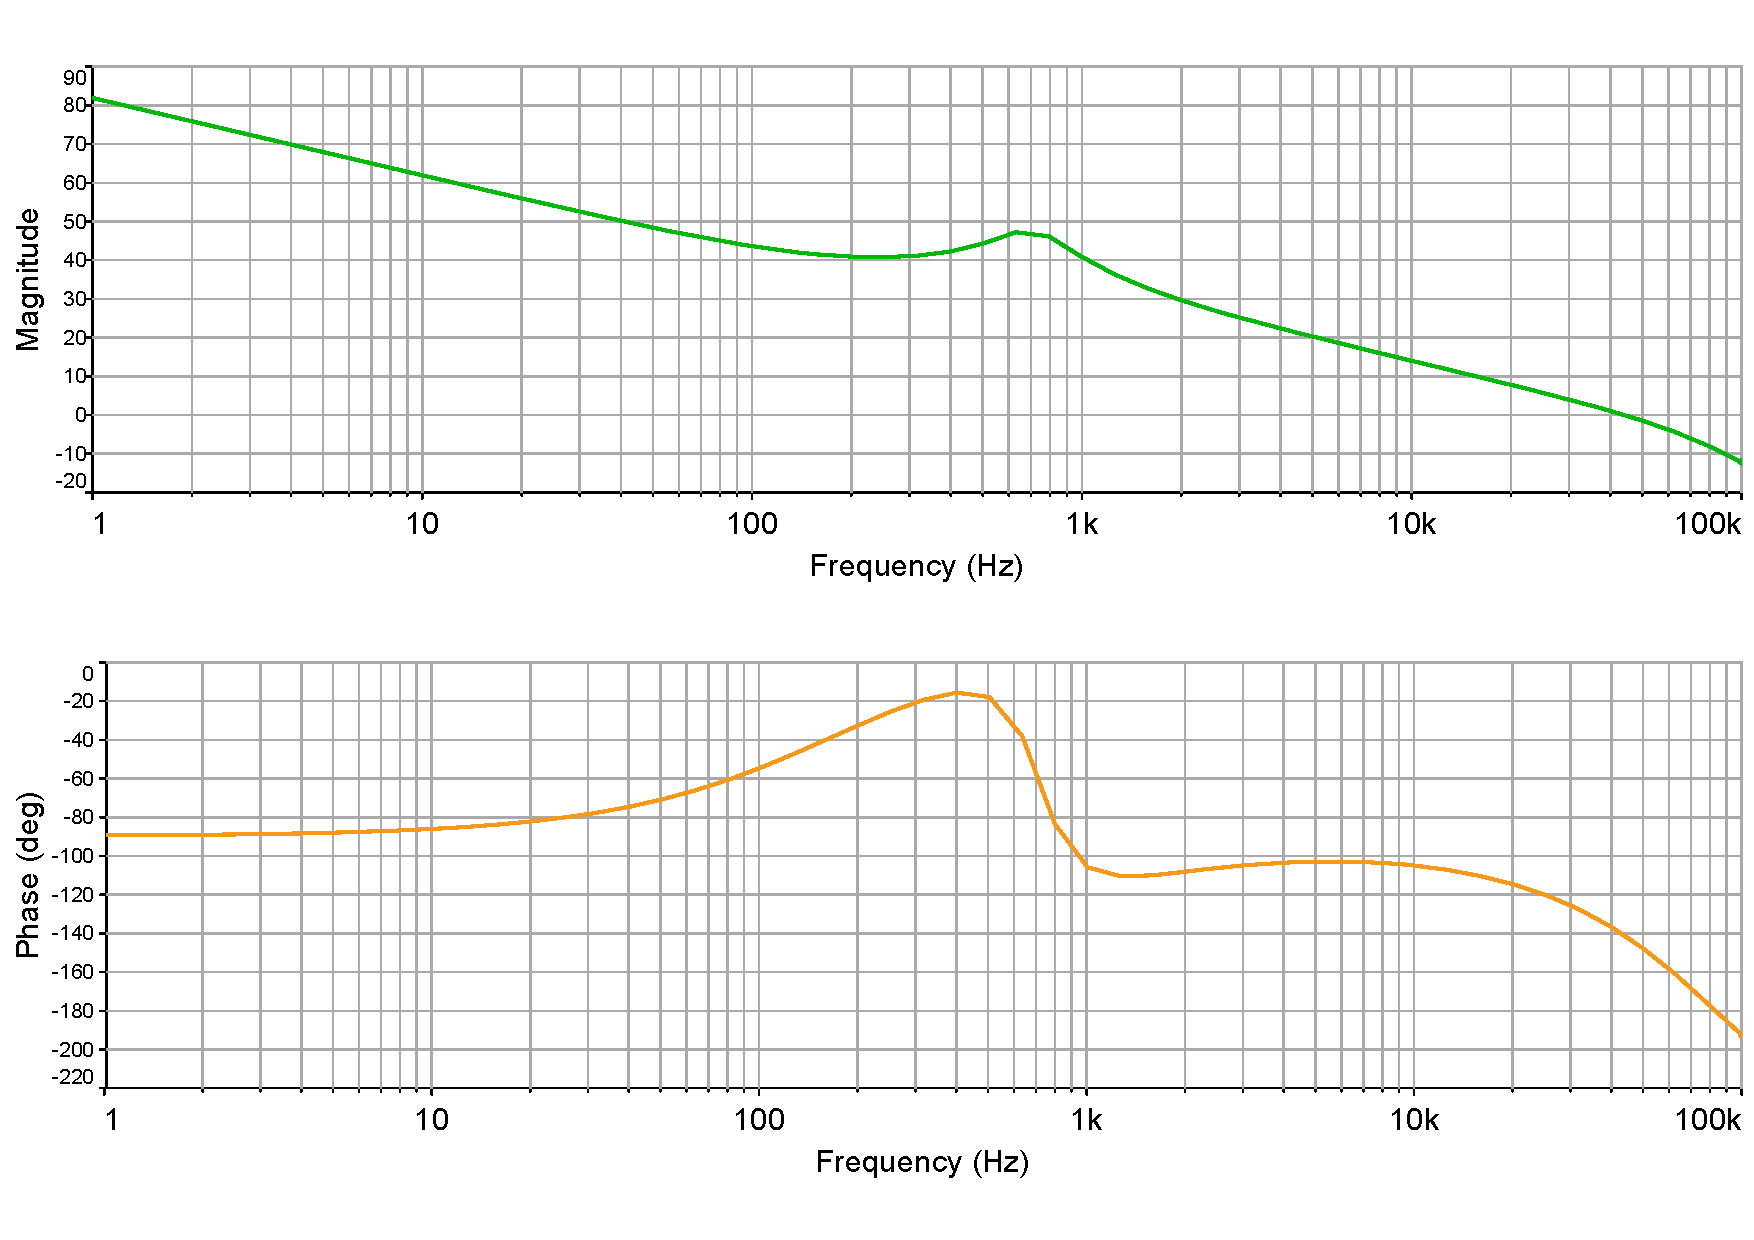
\includegraphics[width=12cm]{BodeGraph.pdf}
  \caption{被自动翻转的bode图}
  \label{rotatedBode}
\end{figure}

问题原因

同一幅图片,XeLaTeX~编译出现图片翻转,而~pdfLaTeX~编译,输出正常。
原因可能是出现在~XeLaTeX~编译过程中会将有些~pdf~文件自身多余的旋转命令编译出来。

问题解决方法

第一种方法(抄自刘海洋大牛的方案):
使用命令\\ \texttt{pdfcrop foo.pdf foo-new.pdf},当然,新文件名可以和旧文件名相同。 这个方法的好处就是 pdfcrop 是texlive自带的,我装的是texlive2017,因此自带了。

第二种方法:采用GhostScript软件消除多余的旋转命令。
\begin{enumerate}
    \item 下载安装~GhostScript~软件,官网为\url{https://www.ghostscript.com/download/gsdnld.html/}
        
    \item 将安装后的bin文件夹地址加入用户环境变量,在我电脑上为~\verb|D:|\verb|\Program Files|\verb|\gs|\verb|\gs9.22|\verb|\bin|
	
    \item cmd~命令行进入想转换图片所在文件夹,执行命令\\gswin32c -sDEVICE=pdfwrite -o newname.pdf  previousname.pdf
              得到一个去除多余旋转命令的~newname.pdf~文件。

    \item 在\LaTeX{}中插入该~pdf~文件,XeLaTeX~编译。
\end{enumerate}

处理之后的图片如图~\ref{Bode}~所示。
\begin{figure}[H] 
  \centering
  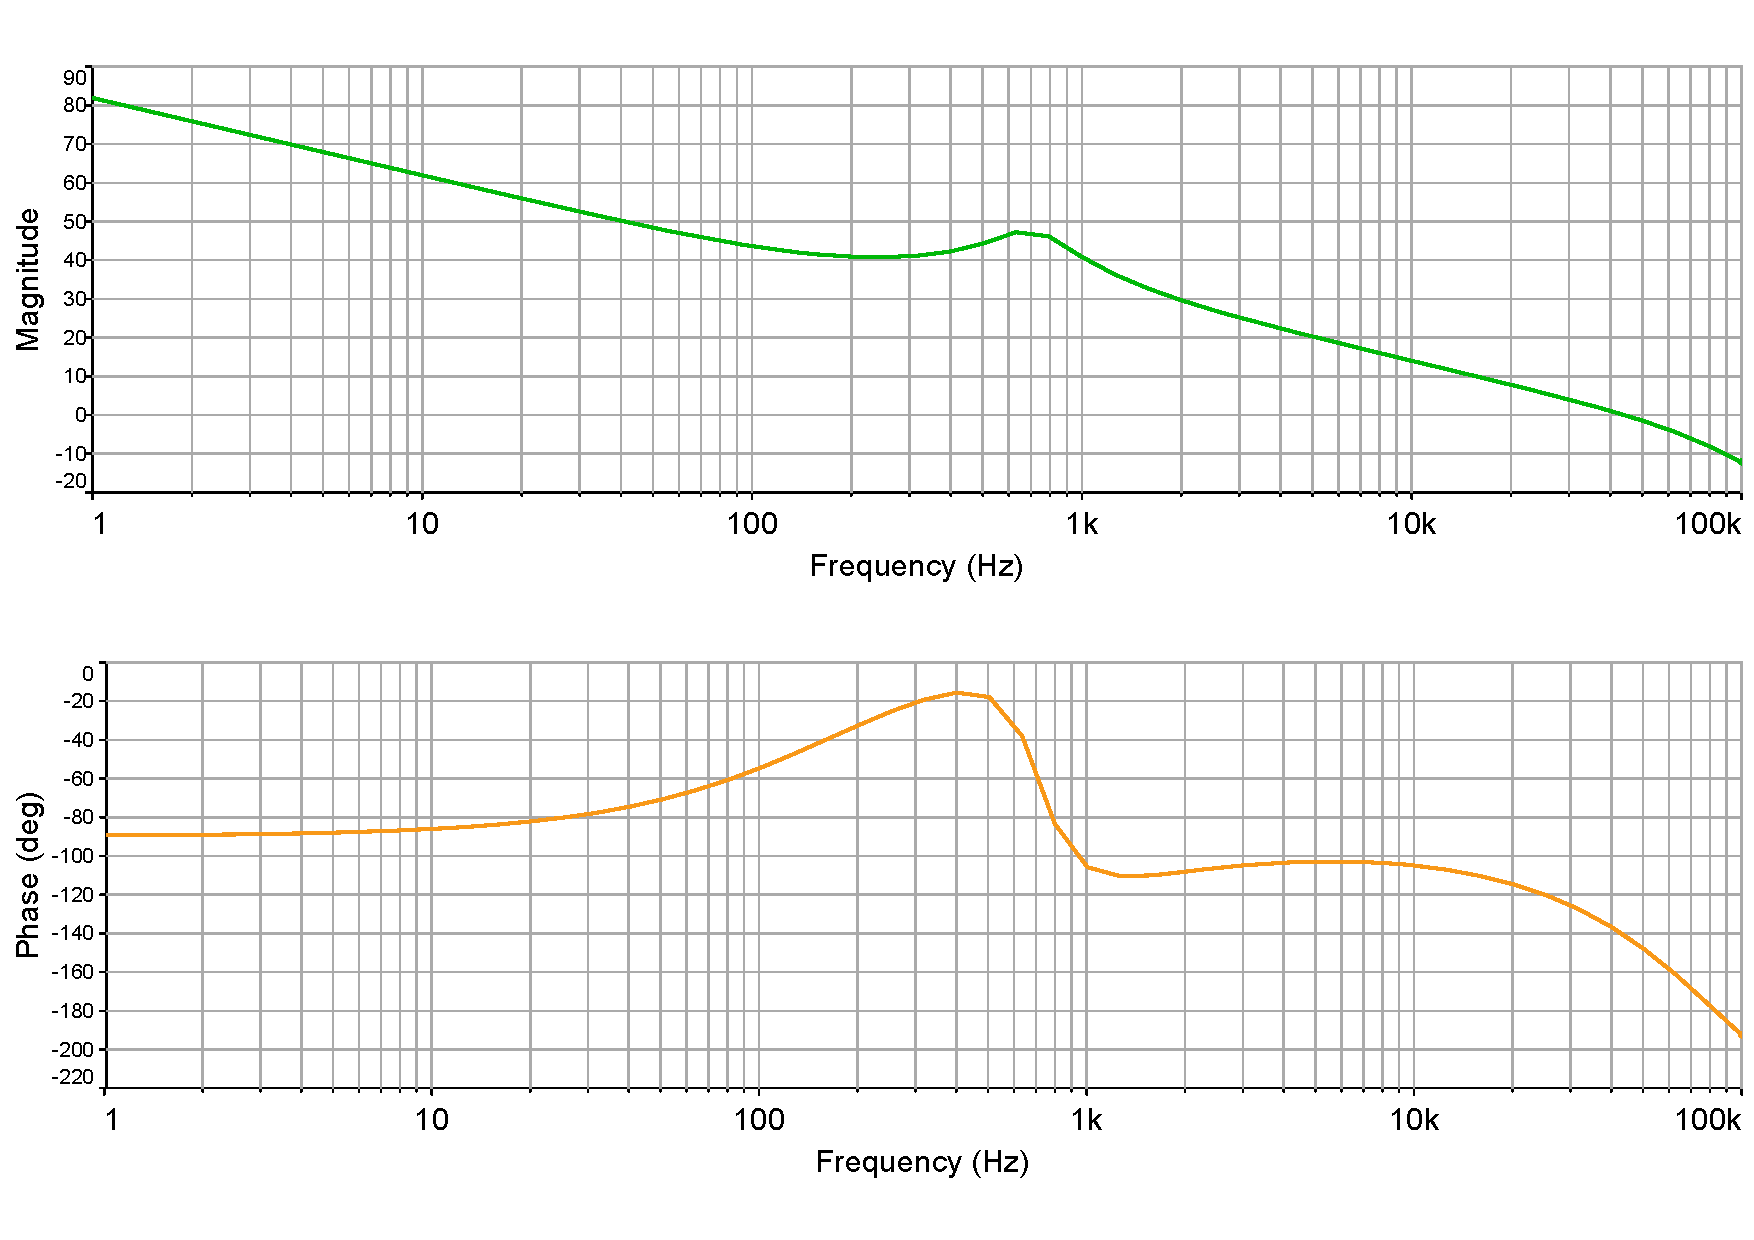
\includegraphics[width=12cm]{Bode.pdf}
  \caption{处理后的bode图}
  \label{Bode}
\end{figure}






\section{网络模型结构}
\subsection*{网络模型结构}
\frame{
  \frametitle{网络整体结构}
	\begin{figure}[h]
		\centering
		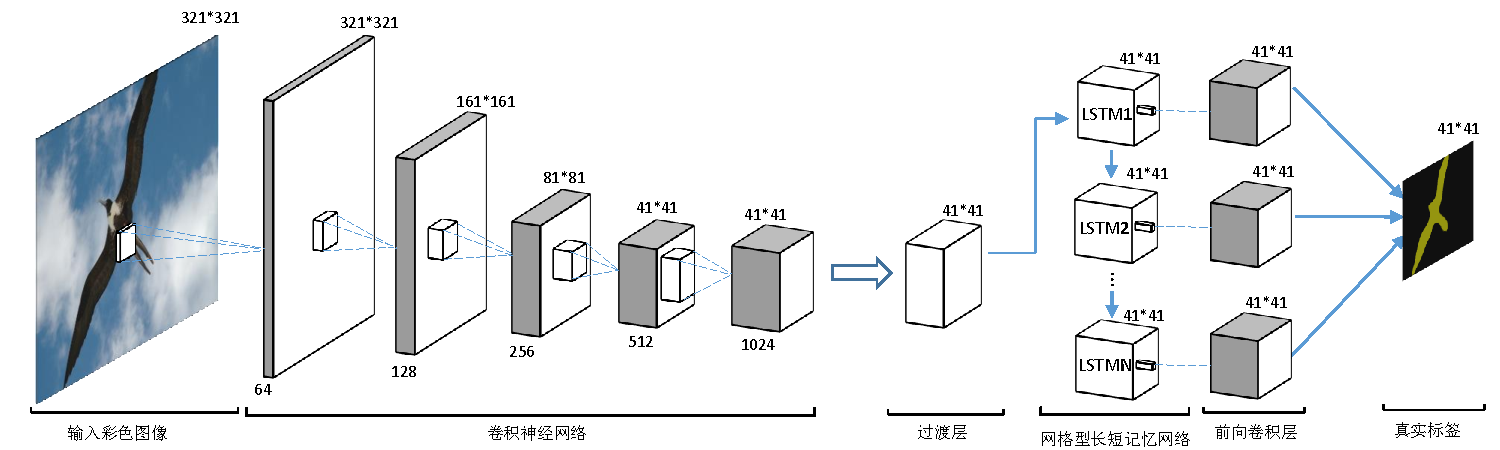
\includegraphics[width=0.9\textwidth,height=0.28\textwidth]{image/illustration/networkstructure.pdf}
		\caption{网络整体结构图}
		\label{fig:networkstructure}
	\end{figure}
	\vspace{-1em}
	\small
	\begin{block}{}
	\begin{itemize}
		\item  四个组成部分:\textbf{卷积网络部分},过渡层,\textbf{网格型长短记忆网络部分},前向卷积层
		\item 核心思想:在卷积网络后堆叠多层网格型长短记忆层
	\end{itemize}
	\end{block}
}
\frame{
	\frametitle{卷积网络部分}
	\vspace{-1em}
	\footnotesize
	\begin{block}{}
	\begin{itemize}
		\item 基于$VGG_{16}$模型\footnote{Simonyan \& Zissermanet, Very deep Convolutional Networks For Large-scale Image Recognition, ICLR 2015}, 含有16层卷积层
		\item 使用了“孔算法”,在不损失精度的情况下将模型参数减少了 6.5 倍\footnote{Chen et al, DeepLab-LargeFOV, ICLR 2015}
	\end{itemize}
	\end{block}
	\vspace{-1em}
	\begin{figure}[h]
		\centering
		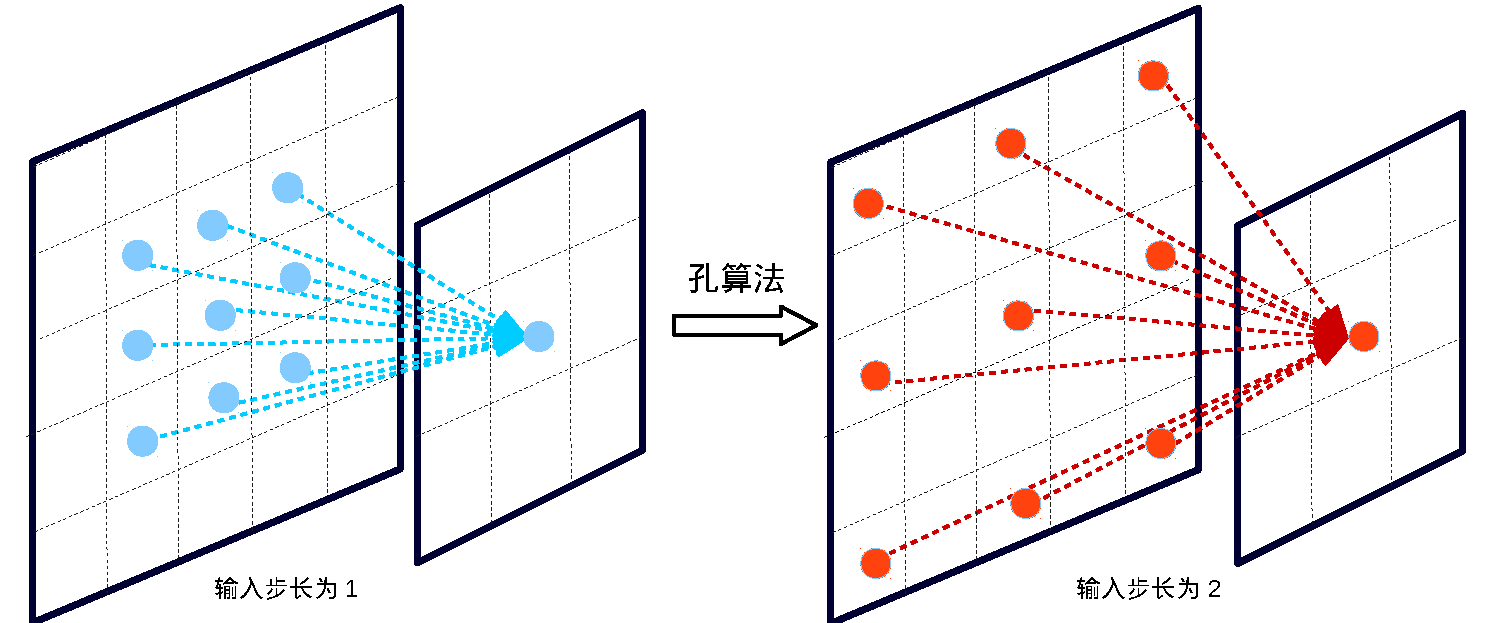
\includegraphics[width=0.7\textwidth]{image/illustration/hole.pdf}
		\caption{"孔算法"示意图}
	\end{figure}
}

\frame{
\frametitle{网格型长短记忆网络部分}
	\vspace{-1em}
    \begin{columns}%[onlytextwidth]
        \begin{column}{0.6\textwidth}
        \vspace{0.2em}
		\begin{figure}
			\centering
			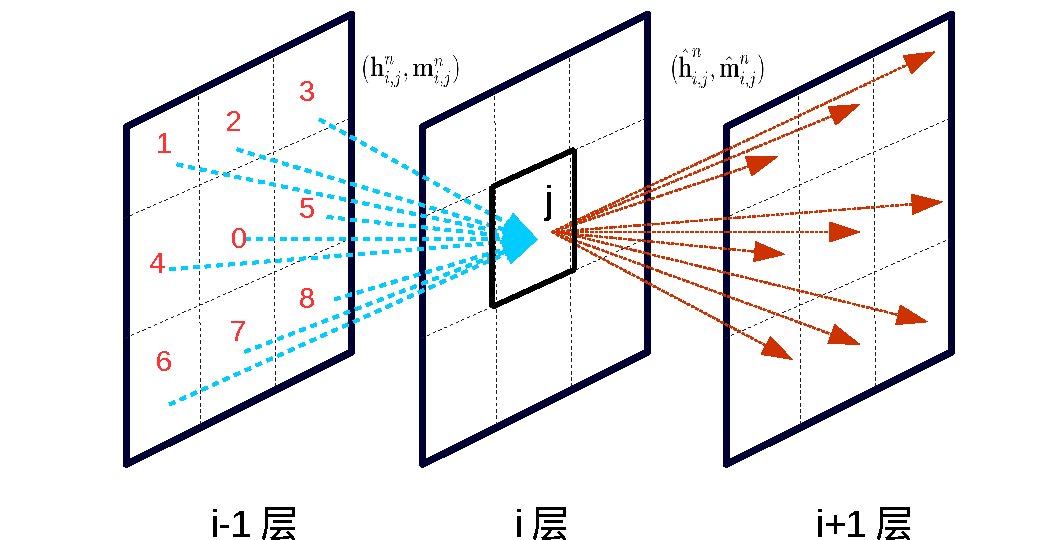
\includegraphics[width=\textwidth]{image/illustration/neighboring.pdf}
			\caption{九维网格型长短记忆网络层之间的通信示意图}
			\label{fig:neighboring}
		\end{figure}
		\end{column} 
		%%%%%%% new column
		\begin{column}{0.5\textwidth}
			\footnotesize
			\vspace{-1.5em}
			\begin{align}
				\begin{split}
				(\hat{\textbf{h}}_{i,j}^0,\hat{\textbf{m}}_{i,j}^0) &= \mbox{LSTM}(\textbf{H}_{i,j},\textbf{m}_{i,j}^0,\textbf{W}_i) \\
				(\hat{\textbf{h}}_{i,j}^1,\hat{\textbf{m}}_{i,j}^1) &= \mbox{LSTM}(\textbf{H}_{i,j},\textbf{m}_{i,j}^1,\textbf{W}_i) \\
				\vdots \\
				(\hat{\textbf{h}}_{i,j}^N,\hat{\textbf{m}}_{i,j}^N) &= \mbox{LSTM}(\textbf{H}_{i,j},\textbf{m}_{i,j}^N,\textbf{W}_i) \\
				\textbf{H}_{i,j} &= [\textbf{h}_{i,j}^0\mbox{ }\textbf{h}_{i,j}^1\mbox{ }...\mbox{ }\textbf{h}_{i,j}^N]^T
				\end{split}
			\end{align}
		\end{column}
    \end{columns}
	\footnotesize
	\vspace{-1em}
	\begin{block}{九维网格型长短记忆网络}
		\vspace{-0.7em}
		\begin{itemize}
			\item 每个位置的预测会受到上一层相邻八邻域特征的影响
			\item 随着层数的堆叠,每一位置将会有更大的感知域。
			\item 网格型长短记忆网络的层数通过实验来确定
		\end{itemize}
	\end{block}
}



\end{code}
\begin{code}
\backmatter
\bibliography{ref/refs}%参考文献

%%% Local Variables:
%%% mode: latex
%%% TeX-master: "../main"
%%% End:

\begin{ack}
  衷心感谢导师 xxx 教授和物理系 xxx 副教授对本人的精心指导。他们的言传身教将使
  我终生受益。

  在美国麻省理工学院化学系进行九个月的合作研究期间,承蒙 xxx 教授热心指导与帮助,不
  胜感激。感谢 xx 实验室主任 xx 教授,以及实验室全体老师和同学们的热情帮助和支
  持!本课题承蒙国家自然科学基金资助,特此致谢。

  感谢 \ucasthesis,它的存在让我的论文写作轻松自在了许多,让我的论文格式规整漂亮了
  许多。
\end{ack}
%致谢

\begin{appendix}%附录
  %%================================================
%% Filename: app01.tex
%% Encoding: UTF-8
%% Author: Yuan Xiaoshuai - yxshuai@gmail.com
%% Created: 2012-04-25 15:16
%% Last modified: 2016-08-28 21:06
%%================================================
\newgeometry{left=2cm,top=3cm,bottom=2cm,right=2cm,includefoot}
\chapter{表格附件}
\section*{\centering\sanhao\hei 毕业设计(论文)任务书}
\addcontentsline{toc}{section}{附表~1:毕业设计(论文)任务书}
\vspace*{.5ex}
\begin{center}
\renewcommand\arraystretch{1.25}
\newcommand{\minitab}[2][>{\rm}m{2em}]{\begin{tabular}{#1}#2\end{tabular}}
\begin{tabularx}{\textwidth}{|>{\centering\rm}m{2em}|X|}
\hline
\multirow{6}{2em}{\minitab{课\\题\\情\\况}} &
\minitab[>{\centering\rm}m{7em}|c]{课题名称 & } \\ 
\cline{2-2}
&\minitab[>{\centering\rm}m{7em}|>{\centering}m{3em}|>{\centering\rm}m{2em}|>{\centering}m{2em}|>{\centering\rm}m{2em}|>{\centering}m{2em}|>{\centering\rm}m{3em}|X]{
教师姓名 & & 职称 & & 学位 & & 教研室 & }\\
\cline{2-2}
 & \minitab[>{\centering\rm}m{7em}|>{\rm}c]{课题来源 & A. 科研 \checkmark\quad B. 生产\quad C. 教学\quad D. 其它}\\
\cline{2-2}
 &\minitab[>{\centering\rm}m{7em}|>{\centering\rm}m{12em}|>{\centering\rm}m{4em}|X]{课题类别 & A. 设计\quad B. 论文 \checkmark & 实施地点 & }\\
\cline{2-2}
 &
\minitab[>{\centering\rm}m{7em}|>{\centering}m{12em}|>{\centering\rm}m{4em}|>{\rm}X]{起止时间 & 2011 年 11 月 $\sim$ 2012 年 6 月 & 上机时数 & }\\
\cline{2-2}
 & \minitab[>{\centering\rm}m{7em}|>{\rm}X]{拟指导的学生数 & \minitab[c|>{\rm}c|c]{1 人 & 对学生的特殊要求 & 基础知识扎实,动手能力较强}}\\
\hline
{\renewcommand\arraystretch{1}\minitab{主\\要\\研\\究\\内\\容}}&{
\vspace*{-7ex}\begin{minipage}[t][10ex][s]{.9\textwidth}\hspace{2em}
主要研究内容
\end{minipage}
}\\
\hline
{\renewcommand\arraystretch{1}\minitab{目\\标\\和\\要\\求}} &{
\vspace*{-6.4ex}\begin{minipage}[t][10ex][s]{.9\textwidth}\hspace{2em}
目标和要求
\end{minipage}
}\\
\hline
{\renewcommand\arraystretch{1}\minitab{特\\色}} & 特色\\
\hline
{成果形式} & 论文\\
\hline
{成果价值} & 有一定的学术价值\\
\hline
{\renewcommand\arraystretch{1}\minitab{科\\室\\审\\题\\意\\见}} &
{\rm\vspace*{2.4ex}\hbox{\hspace{.2\textwidth}负责人签字:\hspace{8em}年\hspace{2em}月\hspace{2em}日}}
\\
\hline
{\renewcommand\arraystretch{1}\minitab{学\\院\\审\\批\\意\\见}} &
{\rm\vspace*{2.4ex}\hbox{\hspace{.2\textwidth}主管院长签字:\hspace{7em}年\hspace{2em}月\hspace{2em}日}}
\\
\hline
\end{tabularx}
\end{center}

\newpage
\renewcommand\arraystretch{1.25}
\section*{\centering\song\sanhao 郑州大学毕业论文开题报告表}
\addcontentsline{toc}{section}{附表~2:郑州大学毕业论文开题报告表}
\begin{center}
\vspace*{0.5ex}
\hfil 院(系):\texttt{材料科学与工程学院}\hspace{15em} 类别:论文\hfil\hfil
\vspace*{0.5ex}

\begin{tabularx}{\textwidth}{|>{\centering\rm}p{.12\textwidth}|>{\centering}p{.12\textwidth}|>{\centering\rm}p{.08\textwidth}|>{\centering}p{.15\textwidth}|>{\centering\rm}p{.05\textwidth}|Z|}
\hline
课题名称 & \multicolumn{5}{c|}{} \\
\hline
导师姓名 & & 职\quad{}称 & \multicolumn{3}{c|}{} \\
\hline
学生姓名 & & 学\quad{}号 & & 专业 & \\
\hline
\multicolumn{6}{|c|}{
\begin{minipage}[c]{.96\textwidth}
\vskip 1ex
\textrm{开题报告内容:}(调研资料的准备,选题依据、目的、要求;毕业论文进度安
排;完成毕业论文所需要实验条件等、主要参考文献与资料情况等)\CJKindent

\vspace*{.5ex}
一、选题依据、目的和要求
\vspace*{.5ex}

\vspace*{15ex}

\vspace*{.5ex}
二、实验和检测方法
\vspace*{.5ex}

\vspace*{15ex}

\vspace*{.5ex}
三、实验进度安排
\vspace*{.5ex}

\vspace*{15ex}

\vspace*{.5ex}
四、主要参考文献
\vspace*{.5ex}

\vspace*{15ex}

% \begin{enumerate}[{$[$}1{$]$}]
% 
% \item 
% 
% \end{enumerate}

\vskip 5ex
\hfill \textrm{指导教师:}\hspace{.4\textwidth}
\vskip 1.5ex
\hfill \textrm{学\hspace{2em}生:}\hspace{.4\textwidth}
\vskip 1.5ex
\hfill \textrm{年\hspace{2em}月\hspace{2em}日}\hspace{.2\textwidth}
\vspace{1ex}
\end{minipage}}\\
\hline
\end{tabularx}
\end{center}

\newpage

\section*{\centering\sanhao 毕业设计(论文)计划进程表}
\addcontentsline{toc}{section}{附表~3:毕业设计(论文)计划进程表}

\begin{center}
\renewcommand\arraystretch{1.5}
\newcommand{\minitab}[2][>{\rm}c]{\begin{tabular}{#1}#2\end{tabular}}
\begin{tabularx}{\textwidth}{|>{\centering\rm}p{.12\textwidth}|X|}
\hline
学生姓名 & \minitab[c|>{\rm}c|c|>{\rm}c|c|>{\rm}c|c]{\hspace{4em} & 学号 & \hspace{4em} & 教师姓名 & \hspace{4em} & 职称 & \hspace{3em}}\\\hline
题\hspace{2em}目 & {}\\\hline
周\hspace{2em}次 & {\hfil\textrm{工作内容}\hfil}\\\hline
 & \\
1 $\sim$ 8 周 & \\
9 $\sim$ 10 周 & \\
11 $\sim$ 16 周 & \\
17 $\sim$ 18 周 & \\
19 $\sim$ 21 周 & \\
22 $\sim$ 23 周 & \\
24 周 & \\
 & \begin{minipage}[c]{\textwidth}
\vspace{64ex}
\end{minipage}\\\hline
\end{tabularx}
\end{center}

\newpage
\section*{\centering\sanhao 郑州大学毕业设计中期检查表}
\addcontentsline{toc}{section}{附表~4:郑州大学毕业设计中期检查表}
\begin{center}
\vspace*{0.5ex}
院系:\texttt{材料科学与工程学院}\hfill
\vspace*{0.5ex}

\newcommand{\minitab}[2][>{\rm}c]{\begin{tabular}{#1}#2\end{tabular}}
\begin{tabularx}{\textwidth}{|l|}
\hline
\minitab[>{\rm}c|X]{题\hspace{2em}目 & }\\\hline
\minitab[>{\rm}c|c|>{\rm}c|c]{导师姓名 & \hspace{3em} & 职称 & \hspace{3em}}\\\hline
\minitab[>{\rm}c|c|>{\rm}c|c|>{\rm}c|c]{学生姓名 & \hspace{3em} & 学号 & \hspace{5em} 
& 专业 & \hspace{6em}}\\\hline
\begin{minipage}[c]{.96\textwidth}
\vskip 2ex 
\textrm{一、阶段性成果}
\vskip 1ex\CJKindent

\vspace*{15ex}

\vspace{20ex}
\end{minipage}\\\hline
\begin{minipage}[c]{.96\textwidth}
\vskip 2ex
\textrm{二、存在问题及解决方法}
\vskip 1ex\CJKindent

\vspace*{15ex}

\vskip 1ex
解决方法:
\vskip 1ex

\vskip 20ex
\hfill \textrm{指导教师:}\hspace{.4\textwidth}
\vskip 1.5ex
\hfill \textrm{学\hspace{2em}生:}\hspace{.4\textwidth}
\vskip 1.5ex
\hfill \textrm{年\hspace{2em}月\hspace{2em}日}\hspace{.2\textwidth}
\vspace{2ex}
\end{minipage}\\\hline
\end{tabularx}
\end{center}

\newpage
\section*{\centering\sanhao 毕业设计(论文)成绩评定表}
\addcontentsline{toc}{section}{附表~5:毕业设计(论文)成绩评定表}
\begin{center}
\vspace*{.5ex}
\hspace{4em}学院:\texttt{材料科学与工程学院}\hfill 班级:\hspace{6em}
\vspace*{1ex}

\renewcommand\arraystretch{1.5}
\newcommand{\minitab}[2][>{\rm}c]{\begin{tabular}{#1}#2\end{tabular}}
\begin{tabularx}{\textwidth}{!{\vrule width1.5bp}>{\centering\rm}Z|>{\centering}p{6em}|>{\rm}Z|>{\centering}p{8em}|>{\rm}Z|>{\centering}p{5em}!{\vrule width1.5bp}}
\Xhline{1.5bp}
姓名 & & 学号 & & 总成绩 & \\\hline
题目 & \multicolumn{5}{c!{\vrule width1.5bp}}{}\\\hline
\multirow{8}{3em}{% \renewcommand\arraystretch{1}
  \minitab{指\\导\\老\\师\\评\\语}} &
  \multicolumn{5}{>{\rm}c!{\vrule width1.5bp}}{\multirow{5}*{}}\\
  & \multicolumn{5}{>{\rm}c!{\vrule width1.5bp}}{}\\
  & \multicolumn{5}{>{\rm}c!{\vrule width1.5bp}}{}\\
  & \multicolumn{5}{>{\rm}c!{\vrule width1.5bp}}{}\\
  & \multicolumn{5}{>{\rm}c!{\vrule width1.5bp}}{}\\
  & \multicolumn{5}{>{\rm}c!{\vrule width1.5bp}}{}\\
  & \multicolumn{5}{>{\rm}c!{\vrule width1.5bp}}{}\\
  \cline{2-6}
  & \multicolumn{5}{>{\rm}c!{\vrule width1.5bp}}{
\hspace{2em}评定成绩:\hfill 签名:\hfill \hspace{2em}年\hspace{2em}月
\hspace{2em}日\hspace{2em}
}\\
\hline
\multirow{7}{3em}{% \renewcommand\arraystretch{1}
  \minitab{评\\阅\\人\\评\\语}} &
  \multicolumn{5}{>{\rm}c!{\vrule width1.5bp}}{\multirow{5}*{}}\\
  & \multicolumn{5}{>{\rm}c!{\vrule width1.5bp}}{}\\
  & \multicolumn{5}{>{\rm}c!{\vrule width1.5bp}}{}\\
  & \multicolumn{5}{>{\rm}c!{\vrule width1.5bp}}{}\\
  & \multicolumn{5}{>{\rm}c!{\vrule width1.5bp}}{}\\
  & \multicolumn{5}{>{\rm}c!{\vrule width1.5bp}}{}\\
  \cline{2-6}
  & \multicolumn{5}{>{\rm}c!{\vrule width1.5bp}}{
\hspace{2em}评定成绩:\hfill 签名:\hfill \hspace{2em}年\hspace{2em}月
\hspace{2em}日\hspace{2em}
}\\
\hline
\multirow{8}{3em}{% \renewcommand\arraystretch{1}
  \minitab{答\\辩\\小\\组\\评\\语}} &
  \multicolumn{5}{>{\rm}c!{\vrule width1.5bp}}{\multirow{5}*{}}\\
  & \multicolumn{5}{>{\rm}c!{\vrule width1.5bp}}{}\\
  & \multicolumn{5}{>{\rm}c!{\vrule width1.5bp}}{}\\
  & \multicolumn{5}{>{\rm}c!{\vrule width1.5bp}}{}\\
  & \multicolumn{5}{>{\rm}c!{\vrule width1.5bp}}{}\\
  & \multicolumn{5}{>{\rm}c!{\vrule width1.5bp}}{答辩组成员签名\hspace{12em}}\\
  & \multicolumn{5}{>{\rm}c!{\vrule width1.5bp}}{}\\
  \cline{2-6}
  & \multicolumn{5}{>{\rm}c!{\vrule width1.5bp}}{
\hspace{2em}评定成绩:\hfill 签名:\hfill \hspace{2em}年\hspace{2em}月
\hspace{2em}日\hspace{2em}
}\\
\Xhline{1.5bp}
\end{tabularx}
\end{center}
{\wuhao 注:设计(论文)总成绩 = 指导教师评定成绩(30\%) + 评阅人评定成绩(
30\%) +答辩成绩(40\%)}
\restoregeometry

  %%================================================
%% Filename: app02.tex
%% Encoding: UTF-8
%% Author: Yuan Xiaoshuai - yxshuai@gmail.com
%% Created: 2012-05-04 18:51
%% Last modified: 2016-08-28 21:06
%%================================================
\chapter{\sl The Name of the Game}

English words like `technology' stem from a Greek root beginning with
the letters $\tau\epsilon\chi\ldots\,$; and this same Greek word means {\sl
art\/} as well as technology. Hence the name \TeX, which is an
uppercase form of $\tau\epsilon\chi$.

Insiders pronounce the $\chi$ of \TeX\ as a Greek chi, not as an `x', so that
\TeX\ rhymes with the word blecchhh. It's the `ch' sound in Scottish words
like {\sl loch\/} or German words like {\sl ach\/}; it's a Spanish `j' and a
Russian `kh'. When you say it correctly to your computer, the terminal
may become slightly moist.

The purpose of this pronunciation exercise is to remind you that \TeX\ is
primarily concerned with high-quality technical manuscripts: Its emphasis is
on art and technology, as in the underlying Greek word. If you merely want
to produce a passably good document---something acceptable and basically
readable but not really beautiful---a simpler system will usually suffice.
With \TeX\ the goal is to produce the {\sl finest\/} quality; this requires
more attention to detail, but you will not find it much harder to go the
extra distance, and you'll be able to take special pride in the finished
product. 

On the other hand, it's important to notice another thing about \TeX's name:
The `E' is out of kilter. This 
displaced `E' is a reminder that \TeX\ is about typesetting, and it
distinguishes \TeX\ from other system names. In fact, TEX (pronounced
{\sl tecks\/}) is the admirable {\sl Text EXecutive\/} processor developed by
Honeywell Information Systems. Since these two system names are
pronounced quite differently, they should also be spelled differently. The
correct way to refer to \TeX\ in a computer file, or when using some other
medium that doesn't allow lowering of the `E', is to type `TeX'. Then
there will be no confusion with similar names, and people will be
primed to pronounce everything properly.

\section*{References}
\noindent{\itshape NOTE: these references are only for demonstration, they are
  not real citations in the original text.}

\begin{enumerate}[{$[$}1{$]$}]
\item Donald E. Knuth. The \TeX book. Addison-Wesley, 1984. ISBN: 0-201-13448-9
\item Paul W. Abrahams, Karl Berry and Kathryn A. Hargreaves. \TeX\ for the
  Impatient. Addison-Wesley, 1990. ISBN: 0-201-51375-7
\item David Salomon. The advanced \TeX book.  New York : Springer, 1995. ISBN:0-387-94556-3
\end{enumerate}

\end{appendix}

\resumeitem{个人简历:}
\noindent xxxx 年 xx 月 xx 日出生于 xx 省 xx 县。\\
\noindent xxxx 年 9 月考入 xx 大学 xx 系 xx 专业,xxxx 年 7 月本科毕业并获得 xx 学士学位。\\
\noindent xxxx 年 9 月免试进入 xx 大学 xx 系攻读 xx 学位至今。

\resumeitem{发表论文:} % 发表的和录用的合在一起
\begin{enumerate}[{[}1{]}]
\item Yang Y, Ren T L, Zhang L T, et al. Miniature microphone with silicon-
  based ferroelectric thin films. Integrated Ferroelectrics, 2003,
  52:229-235. (SCI 收录, 检索号:758FZ.)
\item 杨轶, 张宁欣, 任天令, 等. 硅基铁电微声学器件中薄膜残余应力的研究. 中国机
  械工程, 2005, 16(14):1289-1291. (EI 收录, 检索号:0534931 2907.)
\item 杨轶, 张宁欣, 任天令, 等. 集成铁电器件中的关键工艺研究. 仪器仪表学报,
  2003, 24(S4):192-193. (EI 源刊.)
\item Yang Y, Ren T L, Zhu Y P, et al. PMUTs for handwriting recognition. In
  press. (已被 Integrated Ferroelectrics 录用. SCI 源刊.)
\item Wu X M, Yang Y, Cai J, et al. Measurements of ferroelectric MEMS
  microphones. Integrated Ferroelectrics, 2005, 69:417-429. (SCI 收录, 检索号
  :896KM.)
\item 贾泽, 杨轶, 陈兢, 等. 用于压电和电容微麦克风的体硅腐蚀相关研究. 压电与声
  光, 2006, 28(1):117-119. (EI 收录, 检索号:06129773469.)
\item 伍晓明, 杨轶, 张宁欣, 等. 基于MEMS技术的集成铁电硅微麦克风. 中国集成电路, 
  2003, 53:59-61.
\end{enumerate}

\resumeitem{研究成果:} % 有就写,没有就删除
\begin{enumerate}[{[}1{]}]
\item 任天令, 杨轶, 朱一平, 等. 硅基铁电微声学传感器畴极化区域控制和电极连接的
  方法: 中国, CN1602118A. (中国专利公开号.)
\item Ren T L, Yang Y, Zhu Y P, et al. Piezoelectric micro acoustic sensor
  based on ferroelectric materials: USA, No.11/215, 102. (美国发明专利申请号.)
\end{enumerate}
%简历

\end{document}
\end{code}

\section{模板选项}
\label{sec:option}

{\noindent\verb|\documentclass[bachelor]{zzuthesis}|}

\begin{itemize}
\item 论文类型:\verb|bachelor|、\verb|master|、\verb|doctor|
% \item \verb|openright|、\verb|openany|
\end{itemize}
论文类型是模板的必选项,在使用该文档类时,必须指定论文类型。其中
\texttt{bachelor}、\texttt{master}、\texttt{doctor} 分别代表本科毕业设计论文、
硕士研究生学位论文、博士研究生学位论文。

\emph{zzuthesis.cls} 中载入book类时默认选项有:\texttt{12pt},\texttt{a4paper}
。此外,当指定\texttt{doctor} 选项时,默认载入 \texttt{openright} 选项,此时文
档章节出现在奇数页,适合双面打印;指定 \texttt{bachelor} 或 \texttt{master} 选
项时,默认载入 \texttt{openany} 选项,用于单面打印。如果需要更改,则需要修改
\emph{zzuthesis.cls} 的定义。

示例文档 \emph{main.tex} 导言区还定义了图形文件的搜索路径,即命令
\verb|\graphicspath{}|。模板 \verb|.cls| 文档中命令:\\
\verb|\DeclareGraphicsExtensions{.pdf,.eps,.png,.jpg,.jpeg}|\\\noindent
定义了搜索图形文件的扩展名。

此外,由于本科论文与研究生论文要求内容及排布次序不同,为了尽量减少更改文档类型
时需要修改的选项,示例文档 \emph{main.tex} 中用到了 \verb|\ifzzu@bachelor| 等
条件判断命令,以自动控制内容的显示及插入次序。由于该命令中含有 \verb|@| 字符,
故在使用该命令前需要先用命令 \verb|\makeatletter| ,之后还要用
\verb|\makeatother| 恢复其定义。事实上,完全可以删除这些不必要的内容。

\section{基本控制命令}

\subsection*{字体}

\verb|\song|、\verb|\fs|、\verb|\kai|、\verb|\hei|、\verb|\cusong|、
\verb|\xingkai|% 、\verb|\vertfont| 
等命令分别用来切换宋体、仿宋、楷体、黑体、粗宋、行楷% 、竖排宋体
等字体。此外,模板还定义了其它一些切换命令,对应关系如下:
\begin{center}
\begin{tabular}{llll}\hline
 \verb|\song| & \verb|\fs| & \verb|\hei| & \verb|\kai| \\\hline
 \verb|\songti| & \verb|\fangsong| & \verb|\heiti| & \verb|\kaiti| \\\hline
\end{tabular}
\end{center}

\subsection*{字号}

\verb|\chuhao| 等命令定义了一组字体大小,分别为:

\begin{center}
\begin{tabular}{lllll}
\hline
\verb|\chuhao|&\verb|\xiaochu|&\verb|\yihao|&\verb|\xiaoyi|&\\
\verb|\erhao|&\verb|\xiaoer|&\verb|\sanhao|&\verb|\xiaosan|&\\
\verb|\sihao|&\verb|\banxiaosi|&\verb|\xiaosi|&\verb|\wuhao|&\verb|\xiaowu|\\
\verb|\liuhao|&\verb|\xiaoliu|&\verb|\qihao|&\verb|\bahao|&\\\hline
\end{tabular}
\end{center}

使用方法为:\verb|\command[<num>]|,其中 \texttt{command} 为字号命令,
\texttt{num} 为行距。比如 \verb|\xiaosi[1.5]| 表示选择小四字体,行距 1.5 倍。

\subsection*{字距}

\verb|\ziju| 更改汉字之间的默认距离,使用格式为 \verb|\ziju{4bp}|,其中的距离只
要是合适的\TeX{}长度即可。

\subsection*{破折号}

\verb|\pozhehao| 中文破折号在 CJK-\LaTeX\ 里没有很好的处理,我们平时输入的都是
两个小短线,比如这样,{\hei 中国——中华人民共和国}。这不符合中文习惯。所以这里
定义了一个命令生成更好看的破折号,不过这似乎不是一个好的解决办法。有同学说不能
用在 \verb|\section{}| 等命令中使用,简单的办法是可以提供一个不带破折号的段标题
:\\
\verb|\section[<没有破折号精简标题>]{<带破折号的标题>}|。

以下命令是为了模板示例文档而定义的,一般不会用到:
\begin{itemize}
  \item \verb|\TeXLive| \TeX{}发行版名称。
  \item \verb|\zzuthesis| 模板名称:用了大体小写,即\zzuthesis{}。
  \item \verb|\version| 模板版本号:当前版本号为\version。
\end{itemize}

\section{封面及版权声明、摘要}
\label{sec:cover}

\subsection*{封面}

封面格式已经在模板中定义,只需填入相应信息即可。
\begin{itemize}
\item 本科毕业设计论文:
  \begin{itemize}
    \item 中文标题 \verb|\ctitle{<title>}|
    \item 英文标题 \verb|\etitle{<title>}|
    \item 指导老师 \verb|\csupervisor{<name>}|
    \item 职称 \verb|\protitle{<title>}|
    \item 学生姓名 \verb|\cauthor{<name>}|
    \item 学号 \verb|\stuno{<number>}|
    \item 专业 \verb|\cmajor{<major>}|
    \item 院系 \verb|\cdepartment{<department>}|
    \item 完成时间 \verb|\cdate{<date>}|
    % \item 提交时间 \verb|\submitdate{<date>}|
  \end{itemize}
\item 硕士学位论文:
  \begin{itemize}
    \item 学校代码 \verb|\schoolcode{<number>}|
    \item 学号或申请号 \verb|\id{<number>}|
    \item 密级 \verb|\secretlevel{<level>}|
    \item 中文标题 \verb|\ctitle{<title>}|
    \item 作者姓名 \verb|\cauthor{<name>}|
    \item 导师姓名 \verb|\csupervisor{<name>}|
    \item 职称 \verb|\protitle{<title>}|
    \item 学科门类 \verb|\csubject{<subject>}|
    \item 专业名称 \verb|\cmajor{<major>}|
    \item 培养院系 \verb|\cdepartment{<department>}|
    \item 完成时间 \verb|\cdate{<date>}|
  \end{itemize}
\item 博士学位论文需要填入的信息无“培养院系”命令,其它与硕士相同。
\item 硕士与博士学位论文英文封面需填入的信息相同,均为:
  \begin{itemize}
    \item 英文题目 \verb|\ctitle{<title>}|
    \item 作者 \verb|\eauthor{<name>}|
    \item 导师 \verb|\esupervisor{<name>}|
    \item 专业 \verb|\emajor{<major>}|
    \item 院系 \verb|\edepartment{<department>}|\footnote{《规范》中仅提供一个英文封面,博士似乎不应有此项信息。
}
    \item 时间 \verb|\edate{<date>}|。
  \end{itemize}
\end{itemize}
以上信息及相应命令在 \emph{data/cover.tex} 均有示例,使用时一般也应在该文件中
修改。% 其中,模板默认本科论文中提交时间为当前日期,研究生论文中完成时间也默认为
% 当前日期,其它命令默认为空。

版权声明在 \emph{zzuthesis.cfg} 中定义,内容及格式已固定,一般不需要修改,也
没有需要填入的信息。

\subsection*{摘要}

\begin{code}
\begin{cabstract}
 摘要请写在这里...
\end{cabstract}
\begin{eabstract}
 here comes English abstract...
\end{eabstract}
\end{code}

摘要标题的定义用命令:\\
\verb|\zzu@chapter*[tocline]{title}[header]|\\\noindent
该命令通过两个可选项\texttt{tocline} 和 \texttt{header} ,可以控制标题是否在目
录或者页眉中出现,非常强大。该模板中目录、图和附表清单、参考文献、符号说明、致
谢、附录、个人简历等标题的定义均用到了该命令。

\subsection*{关键词}

关键词用英文逗号分割写入相应的命令中,模板会解析各关键词并生成符合不同论文格式
要求的关键词格式。
\begin{code}
\ckeywords{关键词 1, 关键词 2}
\ekeywords{keyword 1, key word 2}
\end{code}

\section{正文章节}
\label{sec:mainbody}

论文各章节标题的格式分别通过重新定义 \verb|\chapter{}| 、 \verb|\section{}| 、
\verb|\subsection{}| 和 \verb|\subsubsection{}| 命令实现。

论文正文部分字号与行距的定义通过对文档类中 \verb|\normalsize| 命令修改而得到;
其中本科论文要求行距为1.25倍,但由于\LaTeX{}中行距的定义与Word中存在区别,行
距设置为1.25倍时略嫌小,故采取与研究生论文同样的固定20磅行距。

% \section{字体字号}
% \label{sec:fonts}
% 
% 模板中定义的字体有:
% \begin{center}
% \begin{tabular}{cccccc}
% \toprule
% 字体 & 命令 & 字体 & 命令 & 字体 & 命令 \\
% \midrule
% 宋体 & \verb|\song| & 仿宋 & \verb|\fs| & 楷体 & \verb|\kai| \\
% 黑体 & \verb|\hei| & 粗宋 & \verb|\cusong| & 行楷 & \verb|\xingkai| \\
% \bottomrule
% \end{tabular}
% \end{center}

% 模板中定义的控制字号大小的命令有:
% \begin{center}
% \begin{tabular}{cccccc}
% \toprule
% 字号 & 命令 & 字号 & 命令 & 字号 & 命令\\
% \midrule
% 初号 & \verb|\chuhao[]| & 一号 & \verb|\yihao[]| & 小一 & \verb|\xiaoyi[]| \\
% 二号 & \verb|\erhao[]| & 小二 & \verb|\xiaoer[]| & 三号 & \verb|\sanhao[]| \\
% 小三 & \verb|\xiaosan[]| & 四号 & \verb|\sihao[]| & 半小四 & \verb|\banxiaosi[]| \\
% 小四 & \verb|\xiaosi[]| & 五号 & \verb|\wuhao[]| & 小五 & \verb|\xiaowu[]| \\
% 六号 & \verb|\liuhao[]| & 小六 & \verb|\xiaoliu[]| & 七号 & \verb|\qihao[]| \\
% 八号 & \verb|\bahao[]| & & & & \\
% \bottomrule
% \end{tabular}
% \end{center}
% 以上命令均提供控制相应行距的可选参数,默认参数为1,即单倍行距。\footnote{此处
% 行距较Word中相应行距略小。}

\section{参考文献}
\label{sec:bib}

关于参考文献模板推荐使用\BibTeX{},文献的管理可以用JabRef,可以比较方便地导入
其他格式的文献引用,或者使用 Google 学术搜索也可以很容易地得到 \emph{bib} 格式
的文献引用信息。

模板中使用命令 \verb|\cite{}| 表示上标标注,并另外定义了 \verb|\onlinecite{}|
命令,作为形文中的参考文献标注。下面是示例:

% 关于书的\cite{tex, companion, ColdSources},还有这些\cite{Krasnogor2004e,
% clzs, zjsw},关于杂志的\cite{ELIDRISSI94, MELLINGER96, SHELL02},硕士论文
% \cite{zhubajie, metamori2004},博士论文\cite{shaheshang, FistSystem01},标准
% 文件\cite{IEEE-1363},会议论文\cite{DPMG,kocher99},技术报告\cite{NPB2}。
普通图书
\cite{gxzzzzqlyt1993,jiangyouxu1998,tangxujun1999,zhaokaihua1995,wangang1912,zhaoyaodong1998,crawfprd1995,iflai1977,obrien1994,rood2001,angwen1988}
;论文集、会议录\cite{zglxxh1990,ROSENTHALL1963,GANZHA2000};科技报告
\cite{dtha1990,who1970,ZHANGZHIXIANG1998,CALMS1965};专利文献
\cite{LIUJIALIN1993,hblz2001,KOSEKI2002};专著中的析出文献
\cite{baishunong1998,gjbzjxxflbmyjs1988,hanjiren1985,BUSECK1980,FOURNEY1971,feilisheng1981,MARTIN1996}
;期刊中的析出文献
\cite{libingmu2000,taorengji1984,yzdztbmz1978,MARAIS1992,HEWITT1984};报纸中的
析出文献\cite{Dingwenxiang2000,Zhangtianqing2000};电子文献(包括专著或连续出
版物中析出的电子文献)
\cite{jiangxiangdong1999,xiaoniu2001,CHRISTINE1998,METCALF1995,TURCOTTE1992,Scitor1983}
。

中文参考文献应增加 \texttt{language=``zh''} 字段,以便进行相应处理。另外,这
个\emph{bst} 对中文文献的支持并不是十全十美,如果有不如意的地方,请手动修改
\emph{bbl} 文件。

有时候不想要上标,那么可以这样 \onlinecite{gxzzzzqlyt1993}。

\section{其它部分}
\label{sec:otherparts}

\subsection*{符号对照表}

简单定义的一个 list,跟 description 非常类似,使用方法参见示例文件。带一个可选
参数,用来指定符号列的宽度(默认为 $2.5\,\mathrm{cm}$)。
\begin{code}
\begin{denotation}[1.5cm]
  \item[E] 能量
  \item[m] 质量
  \item[c] 光速
\end{denotation}
\end{code}

\subsection*{目录、图和附表清单}

模板中章节编号深度 \texttt{secnumdepth} 定义为3,即四级编号;目录深度
\texttt{tocdepth} 定义为2,即目录中显示三级标题。在 \emph{main.tex} 文件中使用
命令 \verb|\tableofcontents|可以生成目录。

模板将插图和附表清单分开,使用命令 \verb|\listoffigures| 和 \verb|\listoftables|
可以分别生成插图清单和表格清单,将其插入到期望的位置即可。

目录和插图及附表清单标题的格式分别通过重新定义命令 \verb|\tableofcontents|、
\verb|\listoftables|和 \verb|listoffigures| 实现;目录和清单条目格式的定义均是
利用 \textbf{titletoc} 宏包中\\
\begin{verbatim}
\titlecontents{<section>}[<left>]{<above>}
              {<before with label>}{<before without label>}
              {<filter and page>}[<after>]
\end{verbatim}
命令。

需要注意的是,由于本科论文不要求插图和附表清单,故在重新定义
\verb|\listoftables| 和 \verb|listoffigures| 时将该两条命令定义为空命令,从而
避免本科论文显示插图和附表清单。

\subsection*{简历}

新定义的环境 \texttt{resume},其中可以包含子标题,如发表的学术论文等,用
\verb|\resumeitem{}|命令即可,例子在示例文档 \emph{data/resume.tex}。

\subsection*{附录}

附录会更改默认的 \texttt{chapter} 属性,故所有附录均插入到 \texttt{appendix} 环境中,避免影响后
文内容。
\begin{code}
\begin{appendix}
 %%================================================
%% Filename: app01.tex
%% Encoding: UTF-8
%% Author: Yuan Xiaoshuai - yxshuai@gmail.com
%% Created: 2012-04-25 15:16
%% Last modified: 2016-08-28 21:06
%%================================================
\newgeometry{left=2cm,top=3cm,bottom=2cm,right=2cm,includefoot}
\chapter{表格附件}
\section*{\centering\sanhao\hei 毕业设计(论文)任务书}
\addcontentsline{toc}{section}{附表~1:毕业设计(论文)任务书}
\vspace*{.5ex}
\begin{center}
\renewcommand\arraystretch{1.25}
\newcommand{\minitab}[2][>{\rm}m{2em}]{\begin{tabular}{#1}#2\end{tabular}}
\begin{tabularx}{\textwidth}{|>{\centering\rm}m{2em}|X|}
\hline
\multirow{6}{2em}{\minitab{课\\题\\情\\况}} &
\minitab[>{\centering\rm}m{7em}|c]{课题名称 & } \\ 
\cline{2-2}
&\minitab[>{\centering\rm}m{7em}|>{\centering}m{3em}|>{\centering\rm}m{2em}|>{\centering}m{2em}|>{\centering\rm}m{2em}|>{\centering}m{2em}|>{\centering\rm}m{3em}|X]{
教师姓名 & & 职称 & & 学位 & & 教研室 & }\\
\cline{2-2}
 & \minitab[>{\centering\rm}m{7em}|>{\rm}c]{课题来源 & A. 科研 \checkmark\quad B. 生产\quad C. 教学\quad D. 其它}\\
\cline{2-2}
 &\minitab[>{\centering\rm}m{7em}|>{\centering\rm}m{12em}|>{\centering\rm}m{4em}|X]{课题类别 & A. 设计\quad B. 论文 \checkmark & 实施地点 & }\\
\cline{2-2}
 &
\minitab[>{\centering\rm}m{7em}|>{\centering}m{12em}|>{\centering\rm}m{4em}|>{\rm}X]{起止时间 & 2011 年 11 月 $\sim$ 2012 年 6 月 & 上机时数 & }\\
\cline{2-2}
 & \minitab[>{\centering\rm}m{7em}|>{\rm}X]{拟指导的学生数 & \minitab[c|>{\rm}c|c]{1 人 & 对学生的特殊要求 & 基础知识扎实,动手能力较强}}\\
\hline
{\renewcommand\arraystretch{1}\minitab{主\\要\\研\\究\\内\\容}}&{
\vspace*{-7ex}\begin{minipage}[t][10ex][s]{.9\textwidth}\hspace{2em}
主要研究内容
\end{minipage}
}\\
\hline
{\renewcommand\arraystretch{1}\minitab{目\\标\\和\\要\\求}} &{
\vspace*{-6.4ex}\begin{minipage}[t][10ex][s]{.9\textwidth}\hspace{2em}
目标和要求
\end{minipage}
}\\
\hline
{\renewcommand\arraystretch{1}\minitab{特\\色}} & 特色\\
\hline
{成果形式} & 论文\\
\hline
{成果价值} & 有一定的学术价值\\
\hline
{\renewcommand\arraystretch{1}\minitab{科\\室\\审\\题\\意\\见}} &
{\rm\vspace*{2.4ex}\hbox{\hspace{.2\textwidth}负责人签字:\hspace{8em}年\hspace{2em}月\hspace{2em}日}}
\\
\hline
{\renewcommand\arraystretch{1}\minitab{学\\院\\审\\批\\意\\见}} &
{\rm\vspace*{2.4ex}\hbox{\hspace{.2\textwidth}主管院长签字:\hspace{7em}年\hspace{2em}月\hspace{2em}日}}
\\
\hline
\end{tabularx}
\end{center}

\newpage
\renewcommand\arraystretch{1.25}
\section*{\centering\song\sanhao 郑州大学毕业论文开题报告表}
\addcontentsline{toc}{section}{附表~2:郑州大学毕业论文开题报告表}
\begin{center}
\vspace*{0.5ex}
\hfil 院(系):\texttt{材料科学与工程学院}\hspace{15em} 类别:论文\hfil\hfil
\vspace*{0.5ex}

\begin{tabularx}{\textwidth}{|>{\centering\rm}p{.12\textwidth}|>{\centering}p{.12\textwidth}|>{\centering\rm}p{.08\textwidth}|>{\centering}p{.15\textwidth}|>{\centering\rm}p{.05\textwidth}|Z|}
\hline
课题名称 & \multicolumn{5}{c|}{} \\
\hline
导师姓名 & & 职\quad{}称 & \multicolumn{3}{c|}{} \\
\hline
学生姓名 & & 学\quad{}号 & & 专业 & \\
\hline
\multicolumn{6}{|c|}{
\begin{minipage}[c]{.96\textwidth}
\vskip 1ex
\textrm{开题报告内容:}(调研资料的准备,选题依据、目的、要求;毕业论文进度安
排;完成毕业论文所需要实验条件等、主要参考文献与资料情况等)\CJKindent

\vspace*{.5ex}
一、选题依据、目的和要求
\vspace*{.5ex}

\vspace*{15ex}

\vspace*{.5ex}
二、实验和检测方法
\vspace*{.5ex}

\vspace*{15ex}

\vspace*{.5ex}
三、实验进度安排
\vspace*{.5ex}

\vspace*{15ex}

\vspace*{.5ex}
四、主要参考文献
\vspace*{.5ex}

\vspace*{15ex}

% \begin{enumerate}[{$[$}1{$]$}]
% 
% \item 
% 
% \end{enumerate}

\vskip 5ex
\hfill \textrm{指导教师:}\hspace{.4\textwidth}
\vskip 1.5ex
\hfill \textrm{学\hspace{2em}生:}\hspace{.4\textwidth}
\vskip 1.5ex
\hfill \textrm{年\hspace{2em}月\hspace{2em}日}\hspace{.2\textwidth}
\vspace{1ex}
\end{minipage}}\\
\hline
\end{tabularx}
\end{center}

\newpage

\section*{\centering\sanhao 毕业设计(论文)计划进程表}
\addcontentsline{toc}{section}{附表~3:毕业设计(论文)计划进程表}

\begin{center}
\renewcommand\arraystretch{1.5}
\newcommand{\minitab}[2][>{\rm}c]{\begin{tabular}{#1}#2\end{tabular}}
\begin{tabularx}{\textwidth}{|>{\centering\rm}p{.12\textwidth}|X|}
\hline
学生姓名 & \minitab[c|>{\rm}c|c|>{\rm}c|c|>{\rm}c|c]{\hspace{4em} & 学号 & \hspace{4em} & 教师姓名 & \hspace{4em} & 职称 & \hspace{3em}}\\\hline
题\hspace{2em}目 & {}\\\hline
周\hspace{2em}次 & {\hfil\textrm{工作内容}\hfil}\\\hline
 & \\
1 $\sim$ 8 周 & \\
9 $\sim$ 10 周 & \\
11 $\sim$ 16 周 & \\
17 $\sim$ 18 周 & \\
19 $\sim$ 21 周 & \\
22 $\sim$ 23 周 & \\
24 周 & \\
 & \begin{minipage}[c]{\textwidth}
\vspace{64ex}
\end{minipage}\\\hline
\end{tabularx}
\end{center}

\newpage
\section*{\centering\sanhao 郑州大学毕业设计中期检查表}
\addcontentsline{toc}{section}{附表~4:郑州大学毕业设计中期检查表}
\begin{center}
\vspace*{0.5ex}
院系:\texttt{材料科学与工程学院}\hfill
\vspace*{0.5ex}

\newcommand{\minitab}[2][>{\rm}c]{\begin{tabular}{#1}#2\end{tabular}}
\begin{tabularx}{\textwidth}{|l|}
\hline
\minitab[>{\rm}c|X]{题\hspace{2em}目 & }\\\hline
\minitab[>{\rm}c|c|>{\rm}c|c]{导师姓名 & \hspace{3em} & 职称 & \hspace{3em}}\\\hline
\minitab[>{\rm}c|c|>{\rm}c|c|>{\rm}c|c]{学生姓名 & \hspace{3em} & 学号 & \hspace{5em} 
& 专业 & \hspace{6em}}\\\hline
\begin{minipage}[c]{.96\textwidth}
\vskip 2ex 
\textrm{一、阶段性成果}
\vskip 1ex\CJKindent

\vspace*{15ex}

\vspace{20ex}
\end{minipage}\\\hline
\begin{minipage}[c]{.96\textwidth}
\vskip 2ex
\textrm{二、存在问题及解决方法}
\vskip 1ex\CJKindent

\vspace*{15ex}

\vskip 1ex
解决方法:
\vskip 1ex

\vskip 20ex
\hfill \textrm{指导教师:}\hspace{.4\textwidth}
\vskip 1.5ex
\hfill \textrm{学\hspace{2em}生:}\hspace{.4\textwidth}
\vskip 1.5ex
\hfill \textrm{年\hspace{2em}月\hspace{2em}日}\hspace{.2\textwidth}
\vspace{2ex}
\end{minipage}\\\hline
\end{tabularx}
\end{center}

\newpage
\section*{\centering\sanhao 毕业设计(论文)成绩评定表}
\addcontentsline{toc}{section}{附表~5:毕业设计(论文)成绩评定表}
\begin{center}
\vspace*{.5ex}
\hspace{4em}学院:\texttt{材料科学与工程学院}\hfill 班级:\hspace{6em}
\vspace*{1ex}

\renewcommand\arraystretch{1.5}
\newcommand{\minitab}[2][>{\rm}c]{\begin{tabular}{#1}#2\end{tabular}}
\begin{tabularx}{\textwidth}{!{\vrule width1.5bp}>{\centering\rm}Z|>{\centering}p{6em}|>{\rm}Z|>{\centering}p{8em}|>{\rm}Z|>{\centering}p{5em}!{\vrule width1.5bp}}
\Xhline{1.5bp}
姓名 & & 学号 & & 总成绩 & \\\hline
题目 & \multicolumn{5}{c!{\vrule width1.5bp}}{}\\\hline
\multirow{8}{3em}{% \renewcommand\arraystretch{1}
  \minitab{指\\导\\老\\师\\评\\语}} &
  \multicolumn{5}{>{\rm}c!{\vrule width1.5bp}}{\multirow{5}*{}}\\
  & \multicolumn{5}{>{\rm}c!{\vrule width1.5bp}}{}\\
  & \multicolumn{5}{>{\rm}c!{\vrule width1.5bp}}{}\\
  & \multicolumn{5}{>{\rm}c!{\vrule width1.5bp}}{}\\
  & \multicolumn{5}{>{\rm}c!{\vrule width1.5bp}}{}\\
  & \multicolumn{5}{>{\rm}c!{\vrule width1.5bp}}{}\\
  & \multicolumn{5}{>{\rm}c!{\vrule width1.5bp}}{}\\
  \cline{2-6}
  & \multicolumn{5}{>{\rm}c!{\vrule width1.5bp}}{
\hspace{2em}评定成绩:\hfill 签名:\hfill \hspace{2em}年\hspace{2em}月
\hspace{2em}日\hspace{2em}
}\\
\hline
\multirow{7}{3em}{% \renewcommand\arraystretch{1}
  \minitab{评\\阅\\人\\评\\语}} &
  \multicolumn{5}{>{\rm}c!{\vrule width1.5bp}}{\multirow{5}*{}}\\
  & \multicolumn{5}{>{\rm}c!{\vrule width1.5bp}}{}\\
  & \multicolumn{5}{>{\rm}c!{\vrule width1.5bp}}{}\\
  & \multicolumn{5}{>{\rm}c!{\vrule width1.5bp}}{}\\
  & \multicolumn{5}{>{\rm}c!{\vrule width1.5bp}}{}\\
  & \multicolumn{5}{>{\rm}c!{\vrule width1.5bp}}{}\\
  \cline{2-6}
  & \multicolumn{5}{>{\rm}c!{\vrule width1.5bp}}{
\hspace{2em}评定成绩:\hfill 签名:\hfill \hspace{2em}年\hspace{2em}月
\hspace{2em}日\hspace{2em}
}\\
\hline
\multirow{8}{3em}{% \renewcommand\arraystretch{1}
  \minitab{答\\辩\\小\\组\\评\\语}} &
  \multicolumn{5}{>{\rm}c!{\vrule width1.5bp}}{\multirow{5}*{}}\\
  & \multicolumn{5}{>{\rm}c!{\vrule width1.5bp}}{}\\
  & \multicolumn{5}{>{\rm}c!{\vrule width1.5bp}}{}\\
  & \multicolumn{5}{>{\rm}c!{\vrule width1.5bp}}{}\\
  & \multicolumn{5}{>{\rm}c!{\vrule width1.5bp}}{}\\
  & \multicolumn{5}{>{\rm}c!{\vrule width1.5bp}}{答辩组成员签名\hspace{12em}}\\
  & \multicolumn{5}{>{\rm}c!{\vrule width1.5bp}}{}\\
  \cline{2-6}
  & \multicolumn{5}{>{\rm}c!{\vrule width1.5bp}}{
\hspace{2em}评定成绩:\hfill 签名:\hfill \hspace{2em}年\hspace{2em}月
\hspace{2em}日\hspace{2em}
}\\
\Xhline{1.5bp}
\end{tabularx}
\end{center}
{\wuhao 注:设计(论文)总成绩 = 指导教师评定成绩(30\%) + 评阅人评定成绩(
30\%) +答辩成绩(40\%)}
\restoregeometry

 %%================================================
%% Filename: app02.tex
%% Encoding: UTF-8
%% Author: Yuan Xiaoshuai - yxshuai@gmail.com
%% Created: 2012-05-04 18:51
%% Last modified: 2016-08-28 21:06
%%================================================
\chapter{\sl The Name of the Game}

English words like `technology' stem from a Greek root beginning with
the letters $\tau\epsilon\chi\ldots\,$; and this same Greek word means {\sl
art\/} as well as technology. Hence the name \TeX, which is an
uppercase form of $\tau\epsilon\chi$.

Insiders pronounce the $\chi$ of \TeX\ as a Greek chi, not as an `x', so that
\TeX\ rhymes with the word blecchhh. It's the `ch' sound in Scottish words
like {\sl loch\/} or German words like {\sl ach\/}; it's a Spanish `j' and a
Russian `kh'. When you say it correctly to your computer, the terminal
may become slightly moist.

The purpose of this pronunciation exercise is to remind you that \TeX\ is
primarily concerned with high-quality technical manuscripts: Its emphasis is
on art and technology, as in the underlying Greek word. If you merely want
to produce a passably good document---something acceptable and basically
readable but not really beautiful---a simpler system will usually suffice.
With \TeX\ the goal is to produce the {\sl finest\/} quality; this requires
more attention to detail, but you will not find it much harder to go the
extra distance, and you'll be able to take special pride in the finished
product. 

On the other hand, it's important to notice another thing about \TeX's name:
The `E' is out of kilter. This 
displaced `E' is a reminder that \TeX\ is about typesetting, and it
distinguishes \TeX\ from other system names. In fact, TEX (pronounced
{\sl tecks\/}) is the admirable {\sl Text EXecutive\/} processor developed by
Honeywell Information Systems. Since these two system names are
pronounced quite differently, they should also be spelled differently. The
correct way to refer to \TeX\ in a computer file, or when using some other
medium that doesn't allow lowering of the `E', is to type `TeX'. Then
there will be no confusion with similar names, and people will be
primed to pronounce everything properly.

\section*{References}
\noindent{\itshape NOTE: these references are only for demonstration, they are
  not real citations in the original text.}

\begin{enumerate}[{$[$}1{$]$}]
\item Donald E. Knuth. The \TeX book. Addison-Wesley, 1984. ISBN: 0-201-13448-9
\item Paul W. Abrahams, Karl Berry and Kathryn A. Hargreaves. \TeX\ for the
  Impatient. Addison-Wesley, 1990. ISBN: 0-201-51375-7
\item David Salomon. The advanced \TeX book.  New York : Springer, 1995. ISBN:0-387-94556-3
\end{enumerate}

\end{appendix}
\end{code}

\subsection*{致谢}

用法跟摘要、简历等类似,没什么可说的,看示例:\emph{data/ack.tex}。

\subsection*{注释及文中数量符号}

文中注释采用脚注,命令为 \verb|\footnote{}|,显示格式为\LaTeX{}默认,仅修改了脚
注字体大小及行距,通过对命令 \verb|\footnotesize| 进行修改实现。

量的符号一般为单个拉丁字母或希腊字母,并一律采用斜体($\mathrm{pH}$例外)。为
区别不同情况,可在量符号上附加角标。在表达量值时,在公式、图、表和文字叙述中,
一律使用单位的国际符号,且无例外地用正体。单位符号与数值间要留适当间隙。建议统
一使用公式输入,其中单位需使用 \verb|\mathrm| 命令,单位符号与数值间的间隙用命
令 \verb|$\,$|。示例:量的符号—— \verb|$t_d$|,显示为$t_d$,单位数值——
\verb|$12\,\mathrm{kg}$|,显示为$12\,\mathrm{kg}$。

\subsection*{列表环境}

为了适合中文习惯,模板将 \texttt{itemize}、 \texttt{enumerate} 和
\texttt{description} 三个常用的列表环境
用 \textbf{paralist} 对应的压缩环境替换。一方面减少了多余空间,另一方面可以自
己指定标签的样式和符号。细节请参看\textbf{paralist} 文档,此处不再赘述。示例:
\begin{enumerate}
\item Fedora 16 + \TeXLive{} 2011 + Jabref 2.7.2
  \begin{enumerate}
    \item Fedora 16 + \TeXLive{} 2011 + Jabref 2.7.2
    \item Windows XP + \TeXLive{} 2011 + Jabref 2.7.2
  \end{enumerate}
\item Windows XP + \TeXLive{} 2011 + Jabref 2.7.2
\end{enumerate}
